\documentclass[conference]{IEEEtran}
\IEEEoverridecommandlockouts

\usepackage[UTF8,scheme=plain]{ctex}
\usepackage{amsmath}
\usepackage{amssymb}
\usepackage{array}
\usepackage{booktabs}
\usepackage{cite}
\usepackage{graphicx}
\usepackage{subcaption}
\usepackage{textcomp}
\usepackage{url}
\usepackage[hidelinks]{hyperref}

\graphicspath{{../figures/}}

\newcommand{\R}{\mathbb{R}}
\newcommand{\E}{\mathbb{E}}
\newcommand{\N}{\mathcal{N}}
\newcommand{\Dist}{\operatorname{Dist}}
\newcommand{\wstar}{w_\star}

\begin{document}

\title{Transformer 在上下文学习中实现预条件梯度下降的复现报告}

\author{
\IEEEauthorblockN{Duan Yixuan（段一璇）}
\IEEEauthorblockA{Data Science\\ID: 72542270}
\and
\IEEEauthorblockN{Mingjing XING（刑明静）}
\IEEEauthorblockA{Data Science\\ID: 72542103}
\and
\IEEEauthorblockN{Wenyue Yang（杨文悦）}
\IEEEauthorblockA{Data Science\\ID: 72542268}
\and
\IEEEauthorblockN{Jingwen Luo（罗靖炆）}
\IEEEauthorblockA{Data Science\\ID: 72542176}
}

\maketitle

\begin{abstract}
本文解读并复现 Ahn、Cheng、Daneshmand 和 Sra 发表于 NeurIPS 2023 的论文 \emph{Transformers learn to implement preconditioned gradient descent for in-context learning}。该论文研究的核心问题是：Transformer 是否能通过在随机线性回归任务上的训练，自然学会类似梯度下降的算法，而不仅仅是存在一组人工构造的权重可以模拟梯度下降。从课程主题看，该论文主要对应优化误差与计算复杂度方向，因为有限层 attention 被解释为一种学习到的迭代优化过程；同时它也涉及表达能力，因为线性 attention 可以表达梯度下降类计算；在上下文样本数实验中还体现出少量样本复杂度视角。本文先梳理论文理论机制，再将原论文的结构性证据与本项目的小规模复现实验证据进行对比分析。
\end{abstract}

\begin{IEEEkeywords}
上下文学习，线性 Transformer，预条件梯度下降，优化误差，学习理论
\end{IEEEkeywords}

\section{引言}
上下文学习指 Transformer 在提示词中看到若干输入输出样例后，无需更新参数即可对新查询进行预测的能力。围绕这一现象，一个重要理论问题是：模型是在做模式匹配、隐式贝叶斯推断，还是在执行某种学习到的算法。本文选取的目标论文 \cite{ahn2023preconditioned} 聚焦一个可解析设定：随机线性回归任务被编码为 prompt，并由去掉 softmax 的线性自注意力 Transformer 处理。

该论文的问题不只是“Transformer 能不能表示梯度下降”。已有研究已经展示，某些 Transformer 权重可以被人工构造为执行优化类更新 \cite{akyurek2023learning,von2023transformers}。Ahn 等人的推进点在于训练景观：当模型在随机任务实例上训练时，最优点或近似临界点是否自然具有梯度法结构。论文在若干可解析设定中给出了肯定答案：单层 attention 的全局最优解实现一步预条件梯度下降；在稀疏多层参数约束下，前向传播等价于多步预条件梯度下降；在放宽参数约束后，模型还可以学习变换输入特征，从而改善条件数。

更宽泛的 ICL 文献包括大语言模型 few-shot 能力的经验展示 \cite{brown2020language}、基于 induction heads 的机制解释 \cite{olsson2022context}，以及将 ICL 解释为隐式贝叶斯推断的概率视角 \cite{xie2022bayesian}。架构背景来自 Transformer 本身 \cite{vaswani2017attention}，表达能力研究则说明 attention 模型可以实现很广泛的计算过程 \cite{perez2021attention,wei2022statistically}。在线性回归 ICL 中，Garg 等人展示了 Transformer 能从上下文中学习简单函数类 \cite{garg2022can}；Akyurek 等人和 von Oswald 等人进一步将该行为与梯度下降等经典算法联系起来 \cite{akyurek2023learning,von2023transformers}。线性 attention 还可被解释为 fast-weight programming 机制 \cite{schlag2021linear}。后续单层分析进一步说明，一步梯度式更新在线性 attention 中具有自然性 \cite{mahankali2023one,zhang2023trained}；从优化角度看，预条件思想也与 AdaGrad 等经典自适应梯度方法相关 \cite{duchi2011adaptive}。

该选题与课程中的优化误差和计算复杂度方向最直接相关。模型被分析为一个有限深度计算过程，用 attention 层逐步降低线性回归任务的预测误差。它也涉及逼近误差，因为论文研究线性 Transformer 能表达哪些算法；此外，上下文样本数会影响任务信息量，因此也可从样本复杂度角度作扩展讨论。

为便于表述，本文采用两个简称。\textbf{Paper-scale Structural Evidence (PSE)} 指原论文在其设定规模下给出的官方结构性实验和图像证据。\textbf{Course-scale Reproduction Evidence (CRE)} 指本项目在课程规模下完成的小规模复现和扩展实验。CRE 不用于替代原论文的数值规模，而用于检验相同理论结构是否能在课程项目设置下呈现出一致趋势。

\section{研究问题与核心挑战}
\subsection{研究问题}
该论文研究的是训练后 Transformer 的机制问题：当模型看到大量随机线性回归 prompt 并通过预测损失训练时，训练目标是否会推动模型学到一种可识别的学习算法。这个问题比“Transformer 是否有足够表达能力”更精确。大型架构可能表达许多算法，但学习理论更关心训练到底选择了哪一种算法。

在线性回归 ICL 设定中，模型不是在一个固定数据集上训练，而是在任务分布上训练。每个 prompt 都有不同的真实参数和不同上下文样本。因此，模型必须学习一种可复用过程：从样例中推断当前任务，并预测 query 标签。经典线性回归中存在 OLS、梯度下降、岭回归、预条件梯度下降等多种可能过程。目标论文说明，在其分析的线性 attention 设定中，训练后过程具有预条件梯度下降形式。

\subsection{核心挑战}
第一，Transformer 训练目标关于 attention 权重是非凸的。即使在线性 attention 简化模型中，多层参数也会让目标函数成为高阶矩阵多项式，分析全局最优和临界点都很困难。

第二，ICL 行为具有算法性，而不只是预测性。loss 低本身并不能说明模型采用了哪种机制。不同计算过程可能产生相似预测。因此论文需要检查矩阵结构，例如 $\Sigma^{1/2}A_i\Sigma^{1/2}$ 是否接近单位阵，以区分预条件梯度下降和普通梯度下降。

第三，有效解释必须区分模型容量和训练选择。证明 Transformer 可以模拟梯度下降属于表达能力结论；证明训练后的权重朝梯度法结构移动，则属于优化和计算复杂度层面的结论。这也是该论文适合作为学习理论复现项目的原因。

\begin{table}[!t]
\centering
\caption{论文与课程学习理论主题的对应关系。}
\label{tab:course_fit}
\begin{tabular}{p{0.27\linewidth}p{0.62\linewidth}}
\toprule
主题 & 本项目中的对应关系\\
\midrule
优化误差 & 训练得到的参数可解释为预条件 GD 步骤\\
计算复杂度 & 有限 Transformer 深度对应固定次数优化迭代\\
逼近误差 & 线性 attention 能表达梯度法学习过程\\
样本复杂度 & 更多上下文样本降低任务不确定性\\
\bottomrule
\end{tabular}
\end{table}

\section{问题设定}
\subsection{随机线性回归 Prompt}
每个上下文学习任务都是一个线性回归实例。先采样任务参数 $\wstar \in \R^d$，再采样上下文特征 $x^{(i)}\in\R^d$，标签由
\begin{equation}
y^{(i)} = \langle x^{(i)}, \wstar \rangle,\quad i=1,\ldots,n
\end{equation}
生成。Prompt 包含 $n$ 个带标签样本和一个 query 特征 $x^{(n+1)}$。query 的标签在输入中被置为 $0$，以避免标签泄露。输入矩阵写为
\begin{equation}
Z_0 =
\begin{bmatrix}
x^{(1)} & x^{(2)} & \cdots & x^{(n)} & x^{(n+1)}\\
y^{(1)} & y^{(2)} & \cdots & y^{(n)} & 0
\end{bmatrix}
\in \R^{(d+1)\times(n+1)}.
\end{equation}
其中前 $d$ 行是特征，最后一行是标签。模型目标是根据上下文预测 $\wstar^\top x^{(n+1)}$。

\begin{figure}[!t]
  \centering
  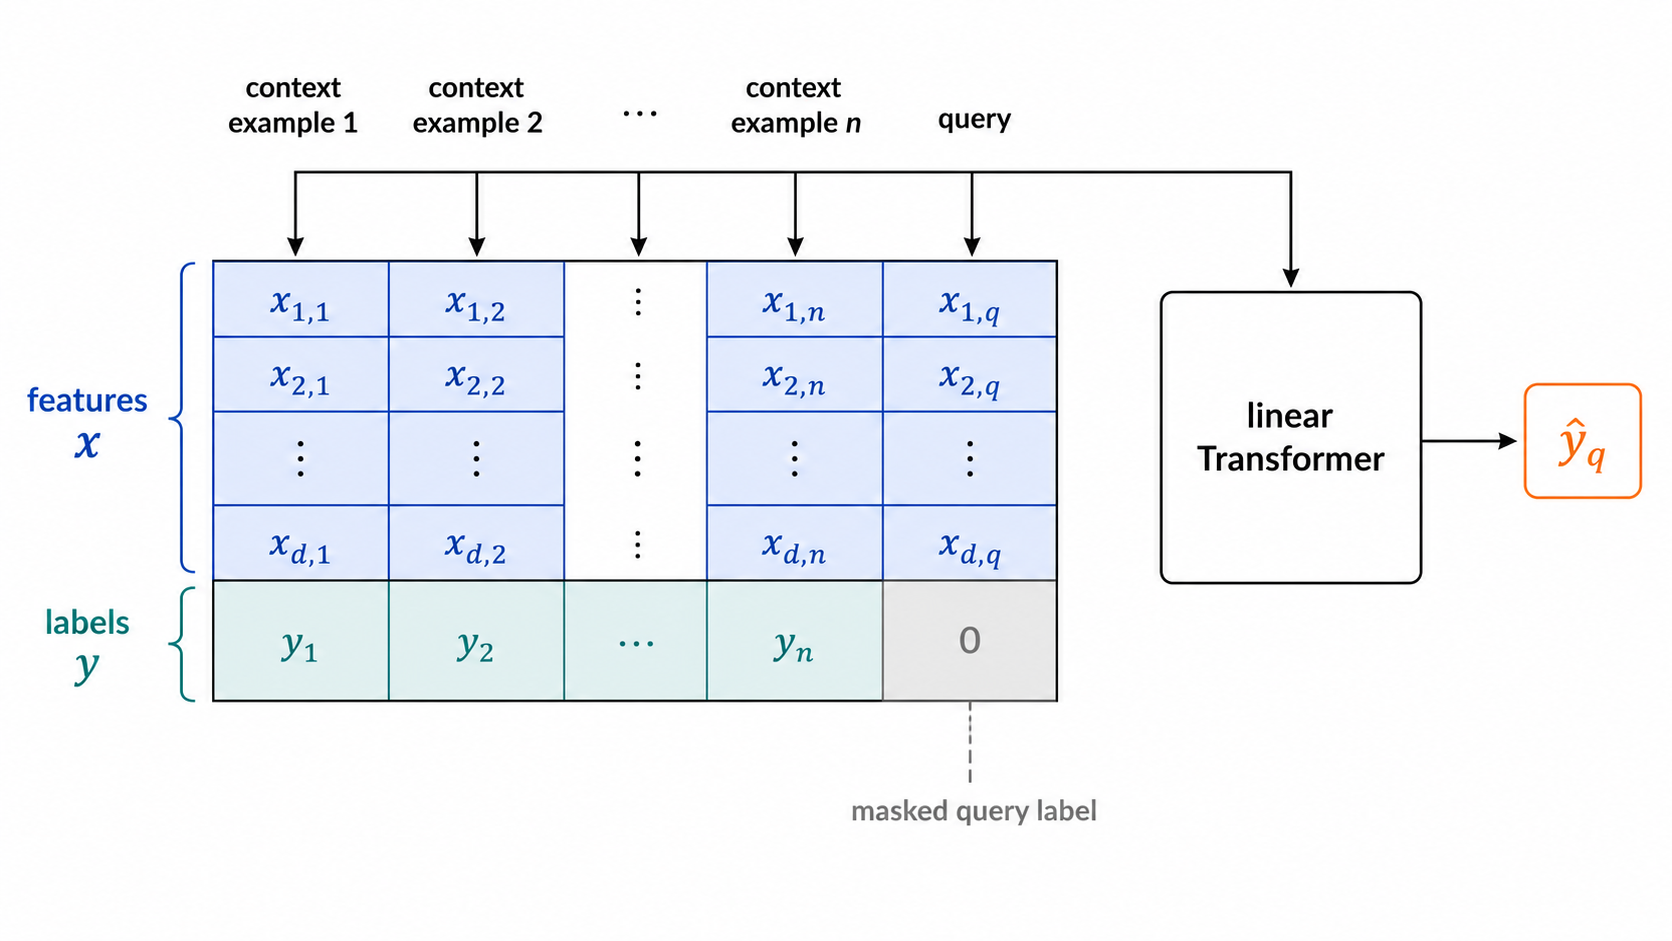
\includegraphics[width=\linewidth]{ai_linear_regression_structure.png}
  \caption{线性回归 prompt 的概念结构。query 标签被 mask，模型必须从上下文样本推断当前任务。}
  \label{fig:ai_prompt}
\end{figure}

\subsection{线性自注意力}
论文为了得到可解析理论，去掉标准 attention 中的 softmax，使用线性 attention。定义 mask
\begin{equation}
M =
\begin{bmatrix}
I_n & 0\\
0 & 0
\end{bmatrix}
\in \R^{(n+1)\times(n+1)}.
\end{equation}
该 mask 保证 attention 只使用带标签的上下文样本。对于可学习矩阵 $P,Q\in\R^{(d+1)\times(d+1)}$，attention 映射为
\begin{equation}
\operatorname{Attn}_{P,Q}(Z)=PZM(Z^\top QZ).
\end{equation}
$L$ 层线性 Transformer 的递推为
\begin{equation}
Z_{\ell+1}=Z_\ell+\frac{1}{n}\operatorname{Attn}_{P_\ell,Q_\ell}(Z_\ell),
\quad \ell=0,\ldots,L-1.
\end{equation}
模型预测定义为
\begin{equation}
\widehat{y}=-[Z_L]_{d+1,n+1}.
\end{equation}
训练目标是在随机 prompt 上的期望平方上下文学习损失。

\section{理论机制}
\subsection{单层全局最优解}
第一个核心结果刻画单层 attention 的全局最优解。当 $x^{(i)}\sim\N(0,\Sigma)$ 且 $\wstar\sim\N(0,I)$ 时，最优 $Q_0$ 的左上角块与协方差矩阵的逆方向一致。在各向同性特例 $\Sigma=I_d$ 中，该解退化为缩放单位阵方向。图 \ref{fig:pse_theorem1} 给出了 PSE 材料中的定理公式。

\begin{figure}[!t]
  \centering
  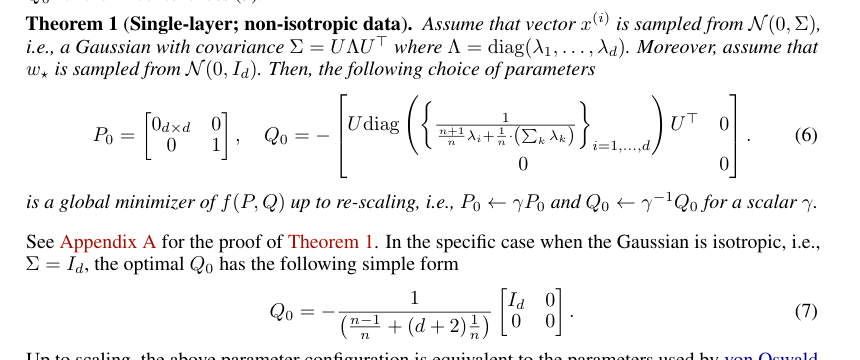
\includegraphics[width=0.95\linewidth]{pse_theorem1_formula.png}
  \caption{PSE 中单层全局最优解的公式。该解对应一步预条件梯度下降。}
  \label{fig:pse_theorem1}
\end{figure}

这个全局最优解具有明确算法含义。线性预测器 $w$ 的经验风险为
\begin{equation}
R_{\wstar}(w)=\frac{1}{2n}\sum_{i=1}^n (w^\top x^{(i)}-\wstar^\top x^{(i)})^2.
\end{equation}
从 $w_0=0$ 出发，一步预条件梯度下降为
\begin{equation}
w_1=w_0-A\nabla R_{\wstar}(w_0)
=\frac{1}{n}A\sum_{i=1}^n y^{(i)}x^{(i)}.
\end{equation}
当 attention 参数取到论文给出的最优形式时，Transformer 的预测等于 $\langle w_1,x^{(n+1)}\rangle$。因此，最优解不仅是一个有效预测器，而且是在执行经典优化步骤。预条件器中的有限样本修正也很重要。当上下文样本数较小时，系数并不只是 $\Sigma^{-1}$，还包含与协方差迹和 $n$ 相关的项。这说明该结果同时具有优化意义和统计意义：模型既适应曲率，也适应上下文不足带来的不确定性。

\subsection{稀疏多层参数约束}
论文随后研究如下稀疏参数形式：
\begin{equation}
P_i =
\begin{bmatrix}
0_{d\times d} & 0\\
0 & 1
\end{bmatrix},
\quad
Q_i =
-
\begin{bmatrix}
A_i & 0\\
0 & 0
\end{bmatrix}.
\end{equation}
在这一约束下，特征行保持不变，标签行被逐层更新。前向传播等价于
\begin{equation}
w_{\ell+1}^{\mathrm{gd}} =
w_\ell^{\mathrm{gd}} - A_\ell \nabla R_{\wstar}(w_\ell^{\mathrm{gd}}),
\quad w_0^{\mathrm{gd}}=0.
\end{equation}
因此，Transformer 的层数可以被解释为优化算法的迭代步数。对于非各向同性输入 $x^{(i)}\sim\N(0,\Sigma)$ 和 $\wstar\sim\N(0,\Sigma^{-1})$，Theorem 3 表明 $A_\ell=a_\ell\Sigma^{-1}$ 形式的参数本质上包含上下文学习损失的临界结构。这是分布级预条件器：当 $n$ 较大时，Hessian $XX^\top/n$ 接近 $\Sigma$，所以 $\Sigma^{-1}$ 能改善条件数。

\subsection{放宽参数约束与特征变换}
Theorem 4 放宽稀疏限制，允许
\begin{equation}
P_i =
\begin{bmatrix}
B_i & 0\\
0 & 1
\end{bmatrix},
\quad
Q_i =
\begin{bmatrix}
A_i & 0\\
0 & 0
\end{bmatrix}.
\end{equation}
对应临界结构满足 $A_i=a_i\Sigma^{-1}$ 且 $B_i=b_iI$。这已经超出标准预条件梯度下降。$A_i$ 负责对标签驱动的梯度步做预条件，$B_i$ 则直接变换特征行，从而近似改善 Gram 矩阵的条件数。这与 von Oswald 等人讨论的 GD++ 机制相联系 \cite{von2023transformers}。

\subsection{为什么该机制并非显然}
这一理论机制并不显然，因为模型训练时并没有收到“执行梯度下降”的指令。它只是在随机 prompt 上最小化预测损失。如果训练后的参数结构与预条件 GD 匹配，就说明训练分布和模型架构隐式诱导出了一种优化算法。因此，论文支持一种算法视角：Transformer 层可以被看作计算步骤，学习到的权重决定这个步骤如何适应数据分布。

这并不意味着所有大语言模型中的每一层都执行同样更新。论文结论更窄但更严格：在受控线性回归设定中，loss landscape 包含具有明确预条件梯度解释的最优点或近似临界结构。这种结论可以通过结构指标进行复现和评估。

\begin{figure}[!t]
  \centering
  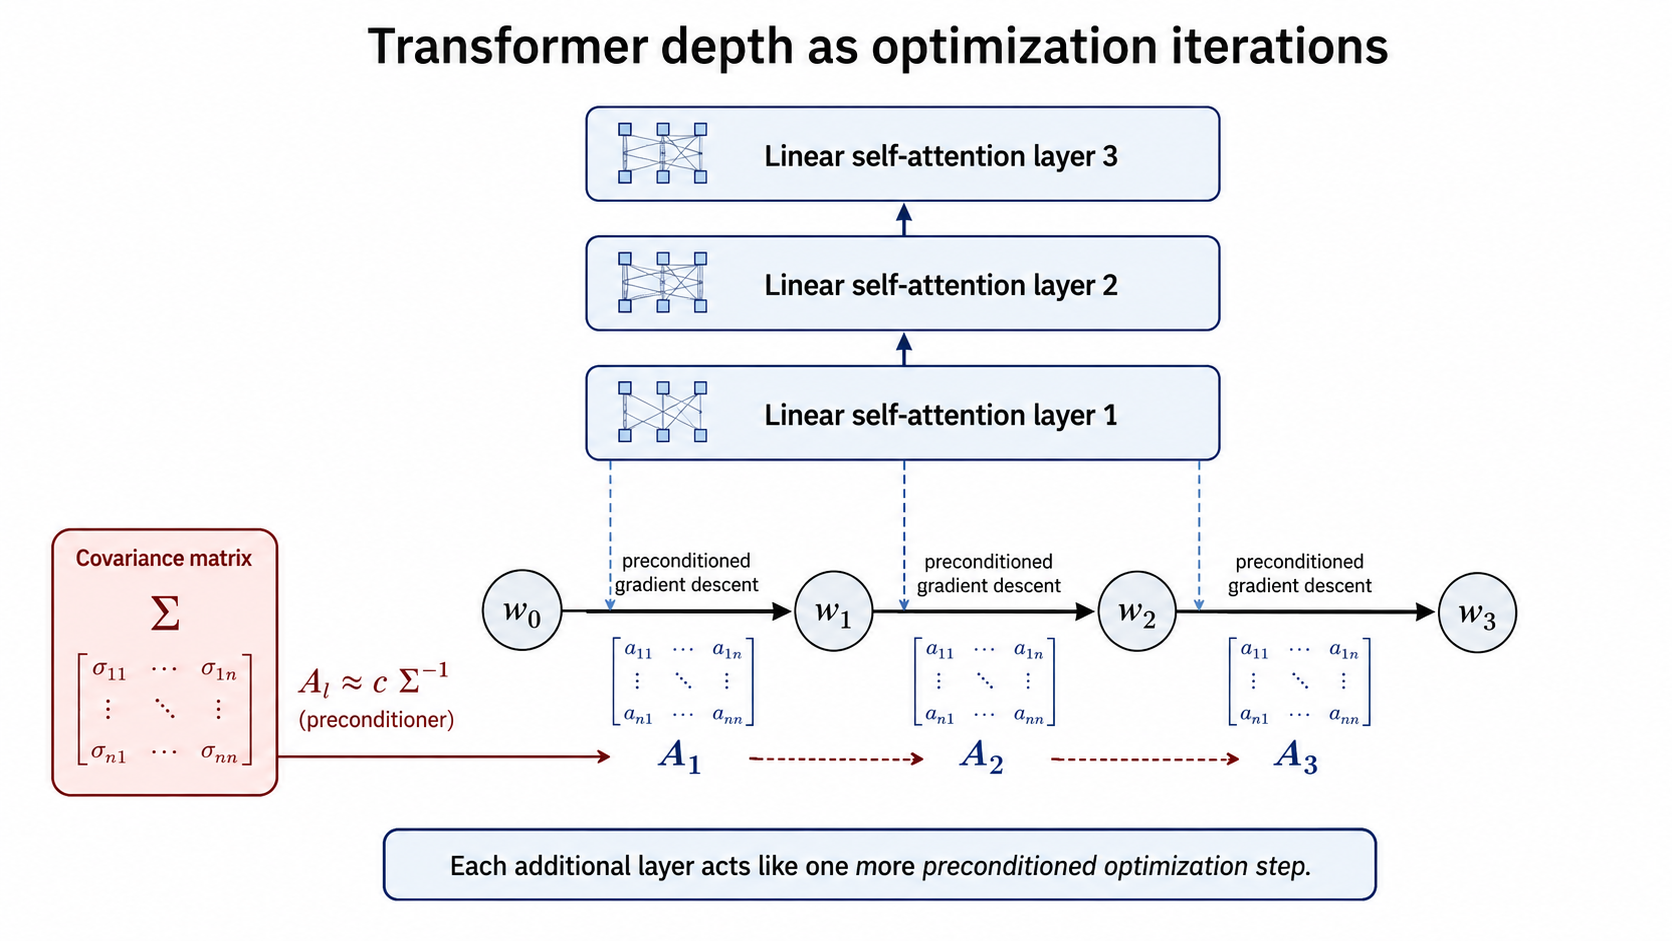
\includegraphics[width=\linewidth]{ai_theoretical_mechanism.png}
  \caption{论文机制的概念图：Transformer 层作为学习到的优化迭代，矩阵参数定义预条件几何。}
  \label{fig:ai_mechanism}
\end{figure}

\subsection{Loss Landscape 解释}
目标论文最理论化的部分不只是前向传播等价性。更强的结论在于随机 prompt 训练目标的 loss landscape。在稀疏参数约束下，模型类别可以被看成 $L$ 步梯度类算法的搜索空间。损失 $f(A)$ 是执行这些学习到的 $L$ 步之后的期望 query 预测误差。Theorem 3 识别出一个结构化集合
\begin{equation}
\mathcal{S}_A=\{A: A_\ell=a_\ell\Sigma^{-1},\ \ell=0,\ldots,L-1\},
\end{equation}
该集合中的点可以具有任意小的梯度范数。这比“存在人工构造权重”更强，因为它将训练目标的驻点结构与经典优化器联系起来；但也比“所有训练都会收敛到该集合”更弱，因此报告中应保留理论表述的精确性。

Theorem 4 在更大的参数空间中进行类似分析。对应结构集合变为
\begin{equation}
\mathcal{S}_{A,B}=\{(A,B):A_\ell=a_\ell\Sigma^{-1},\ B_\ell=b_\ell I\}.
\end{equation}
该集合有双重解释：$A_\ell$ 决定标签残差如何更新隐式预测器，$B_\ell$ 则重塑特征表示。换言之，训练不仅可能学到更新规则，也可能学到一个更易优化的坐标系统。

\subsection{预条件器的统计含义}
预条件器不是任意加速技巧。在高斯线性回归设定中，$\Sigma$ 是输入特征的总体协方差，平方损失的经验 Hessian 与 $XX^\top/n$ 成比例。当 $n$ 较大时，该矩阵集中到 $\Sigma$ 附近，所以 $\Sigma^{-1}$ 近似总体层面的 Newton 方向。当 $n$ 较小时，经验 Hessian 噪声更大且可能病态。单层定理中的有限样本修正项正是捕捉了这一点。因此，该论文也带有样本复杂度意味：同一个预条件器需要同时平衡曲率适应和有限上下文带来的不确定性。

这也解释了为什么报告强调结构指标，而不是只看最终预测 loss。如果 $A_i$ 只是接近 $I$，模型更像普通 GD；如果 $\Sigma^{1/2}A_i\Sigma^{1/2}$ 接近缩放单位阵，则说明 $A_i$ 在合适基底下接近 $\Sigma^{-1}$。后者才是预条件 GD 的理论信号。

\section{推导草图与复现判据}
\subsection{从 Attention 更新到梯度步}
有必要说明稀疏 attention 层为什么会变成梯度步。令 $X=[x^{(1)},\ldots,x^{(n)}]$ 表示上下文特征矩阵，$y=[y^{(1)},\ldots,y^{(n)}]^\top$ 表示标签向量。假设 $Z_\ell$ 的标签行编码了当前预测残差。在稀疏参数约束下，特征行不变，真正起作用的学习矩阵是 $Q_\ell$ 中的 $A_\ell$。由于 mask 只保留上下文列，query 更新依赖 query 特征与上下文特征之间的内积。代数上会出现与下式成比例的项：
\begin{equation}
x^{(n+1)\top}A_\ell X\left(X^\top w_\ell-y\right).
\end{equation}
结合论文中的符号约定和 $1/n$ 缩放，这正是以下更新对 query 预测造成的变化：
\begin{equation}
w_{\ell+1}=w_\ell-A_\ell\frac{1}{n}X(X^\top w_\ell-y).
\end{equation}
右侧向量就是 $\nabla R_{\wstar}(w_\ell)$。因此，在该参数区域中，attention 层并不是比喻意义上“像”梯度下降，而是在代数上等价于一步预条件梯度下降。

\subsection{Mask 与 Query 零标签的作用}
两个实现细节对理论至关重要。mask 防止 query 列作为带标签训练样本参与 attention；query 标签置零则在保持 prompt 矩阵形状的同时避免泄露 $\wstar^\top x^{(n+1)}$。如果改变任一细节，模型对应的就不再是同一个 ICL 目标。因此，在复现项目中，这些不是普通工程细节，而是数学对象的一部分。

符号约定同样重要。预测被定义为 $-[Z_L]_{d+1,n+1}$，所以标签行状态需要带负号解释。如果符号错位，即使架构其他部分正确，表面更新方向也会与梯度下降解释不一致。

\subsection{CRE 能验证什么}
CRE 实验的定位是结构检查。它能验证训练参数是否朝理论预测方向移动，但不能重新证明定理，也不能排除非凸景观中存在其他参数区域。严谨表述应是：复现实验证据通过匹配理论可观测量支持论文结论，而数学保证仍来自原论文分析。

\begin{table}[!t]
\centering
\caption{CRE 使用的结构复现判据。}
\label{tab:criteria}
\begin{tabular}{p{0.20\linewidth}p{0.33\linewidth}p{0.35\linewidth}}
\toprule
结论 & 期望证据 & 可能反例\\
\midrule
Theorem 3 & 旋转 $A_i$ 距离比原始距离下降更明显 & 原始 $A_i$ 接近单位阵但无协方差调整优势\\
Theorem 4 & $B_i$ 与旋转 $A_i$ 距离均下降 & 只有 loss 下降，矩阵保持无结构\\
上下文长度 & 更多样本通常降低测试损失 & 增加上下文后 loss 不改善\\
\bottomrule
\end{tabular}
\end{table}

\subsection{为什么该结果属于计算复杂度视角}
模型层数固定，因此可执行的优化步数也固定。这是一种计算约束。普通梯度下降在病态问题上可能需要很多迭代，而预条件可以减少有效迭代次数。论文结果说明，训练后的 Transformer 可以通过学习协方差感知更新，更有效地利用有限深度。因此，从课程分类看，该论文最适合放在优化误差与计算复杂度方向，而不是只归为表达能力分析。

\section{实验设计}
\subsection{官方证据与复现实验证据}
表 \ref{tab:theory_summary} 总结了与本课程报告最相关的理论结果。图 \ref{fig:pse_summary} 展示了 PSE 材料中的原论文结果总览。

\begin{table}[!t]
\centering
\caption{主要理论结果及其算法解释。}
\label{tab:theory_summary}
\begin{tabular}{p{0.14\linewidth}p{0.30\linewidth}p{0.40\linewidth}}
\toprule
结果 & 模型设定 & 算法解释\\
\midrule
Theorem 1 & 单层线性 attention & 全局最优解实现一步预条件 GD\\
Theorem 3 & 多层稀疏参数 & 临界结构实现 $\Sigma^{-1}$ 预条件 GD\\
Theorem 4 & 放宽 $A_i,B_i$ 参数 & 预条件梯度步加特征变换\\
\bottomrule
\end{tabular}
\end{table}

\begin{figure}[!t]
  \centering
  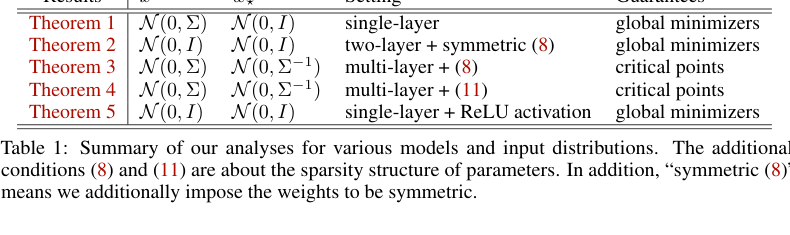
\includegraphics[width=\linewidth]{pse_table1_summary.png}
  \caption{NeurIPS 2023 原论文中不同理论设定的 PSE 总览。}
  \label{fig:pse_summary}
\end{figure}

CRE 实验主要进行三类检查。第一，在 Theorem 3 稀疏约束下，旋转后的矩阵 $\Sigma^{1/2}A_i\Sigma^{1/2}$ 应比原始 $A_i$ 更接近缩放单位阵。第二，在 Theorem 4 放宽约束下，$A_i$ 与 $B_i$ 都应向理论预测结构靠近。第三，上下文长度扩展实验用于观察样本数增加时测试损失如何变化，从而连接样本复杂度视角。

\begin{table}[!t]
\centering
\caption{报告中使用的 CRE 实验设置。}
\label{tab:cre_setup}
\begin{tabular}{p{0.31\linewidth}p{0.55\linewidth}}
\toprule
实验 & 课程规模设置\\
\midrule
Theorem 3 & 三层线性 Transformer，稀疏约束参数，$d=5$，$n=20$，两个随机种子\\
Theorem 4 & 三层放宽线性 Transformer，学习 $A_i$ 和 $B_i$，$d=5$，$n=20$，两个随机种子\\
上下文长度 & $N\in\{4,8,12,16,20\}$，比较 Transformer、GD、PGD 和 OLS\\
\bottomrule
\end{tabular}
\end{table}

\subsection{评价指标}
结构性指标定义为
\begin{equation}
\Dist(M,I)=\min_\alpha \frac{\|M-\alpha I\|_F}{\|M\|_F}.
\end{equation}
Theorem 3 的关键比较是 $\Dist(\Sigma^{1/2}A_i\Sigma^{1/2},I)$ 与 $\Dist(A_i,I)$。如果复现成功，前者应比后者明显下降。Theorem 4 则同时关注旋转后的 $A_i$ 距离和 $\Dist(B_i,I)$。

\section{PSE 与 CRE 结果对比}
\subsection{Theorem 3：稀疏约束下的预条件 GD}
图 \ref{fig:pse_t3} 中的 PSE 结果显示，稀疏约束设置下 loss 下降，旋转距离也下降。关键结论是，训练后的矩阵更接近协方差调整后的 $\Sigma^{-1}$ 方向，而不是原始坐标系中的普通单位阵方向。

\begin{figure}[!t]
  \centering
  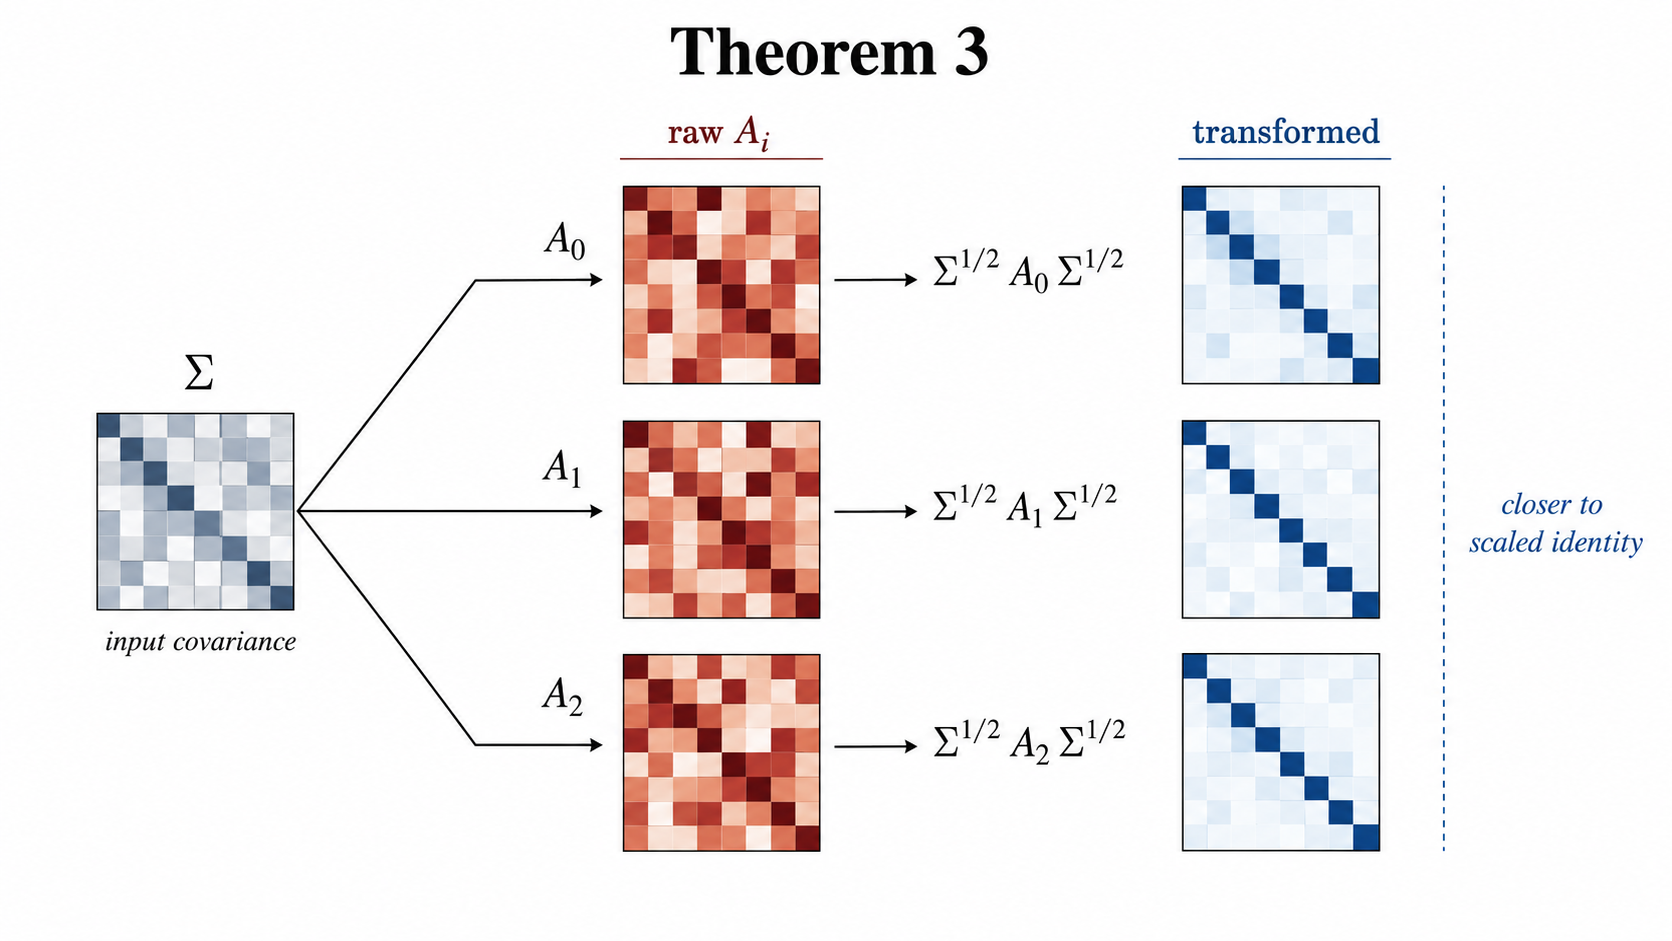
\includegraphics[width=\linewidth]{ai_theorem3_mechanism.png}
  \caption{Theorem 3 机制概念图。稀疏设置检验学习到的 $A_i$ 是否在协方差旋转后对齐 $\Sigma^{-1}$。}
  \label{fig:ai_t3}
\end{figure}

\begin{figure}[!t]
  \centering
  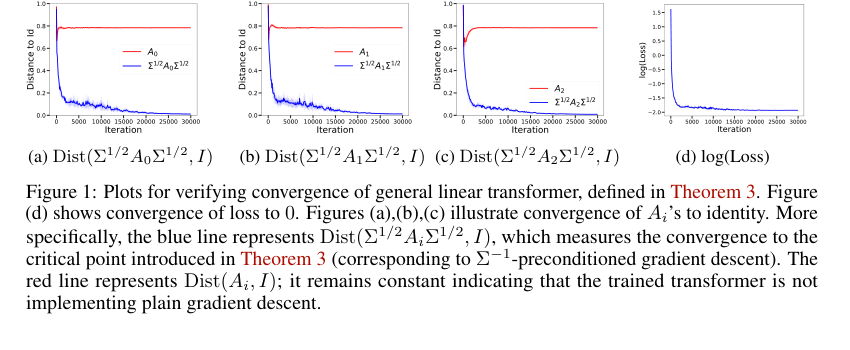
\includegraphics[width=\linewidth]{pse_theorem3_curves.png}
  \caption{Theorem 3 的 PSE 曲线。旋转距离下降，支持 $\Sigma^{-1}$ 预条件器解释。}
  \label{fig:pse_t3}
\end{figure}

CRE 结果遵循相同的结构逻辑。log loss 从 $1.641430$ 降至 $-1.580373$。对于 $A_0$，旋转距离从 $0.950218$ 降至 $0.169304$，而原始距离仅从 $0.999481$ 降至 $0.769688$。$A_1$ 与 $A_2$ 也呈现类似趋势。这说明训练结果更适合解释为协方差感知的预条件器，而不是普通梯度下降。

原始距离与旋转距离的差异是关键。在非各向同性分布中，单位阵并不是理论上最优的更新方向。忽略协方差的方法必须在高方差方向上使用保守步长，因此会浪费低方差方向上的计算效率。预条件方法通过重缩放几何结构，使一层 attention 能表现得像更有效的优化步骤。CRE 结果验证的正是这个理论不变量：经过 $\Sigma^{1/2}$ 旋转后，学习矩阵接近单位阵，而原始矩阵并不需要接近单位阵。

\begin{table}[!t]
\centering
\caption{CRE Theorem 3 结构指标。距离越低表示越接近缩放单位阵。}
\label{tab:t3_metrics}
\begin{tabular}{lrrr}
\toprule
指标 & 初始 & 最终 & 变化\\
\midrule
Log loss & 1.6414 & -1.5804 & -3.2218\\
旋转 $A_0$ 距离 & 0.9502 & 0.1693 & -0.7809\\
原始 $A_0$ 距离 & 0.9995 & 0.7697 & -0.2298\\
旋转 $A_1$ 距离 & 0.9757 & 0.3928 & -0.5830\\
原始 $A_1$ 距离 & 0.9841 & 0.8120 & -0.1721\\
旋转 $A_2$ 距离 & 0.9654 & 0.2126 & -0.7528\\
原始 $A_2$ 距离 & 0.9548 & 0.7573 & -0.1976\\
\bottomrule
\end{tabular}
\end{table}

\begin{figure}[!t]
\centering
\begin{subfigure}{0.48\linewidth}
  \centering
  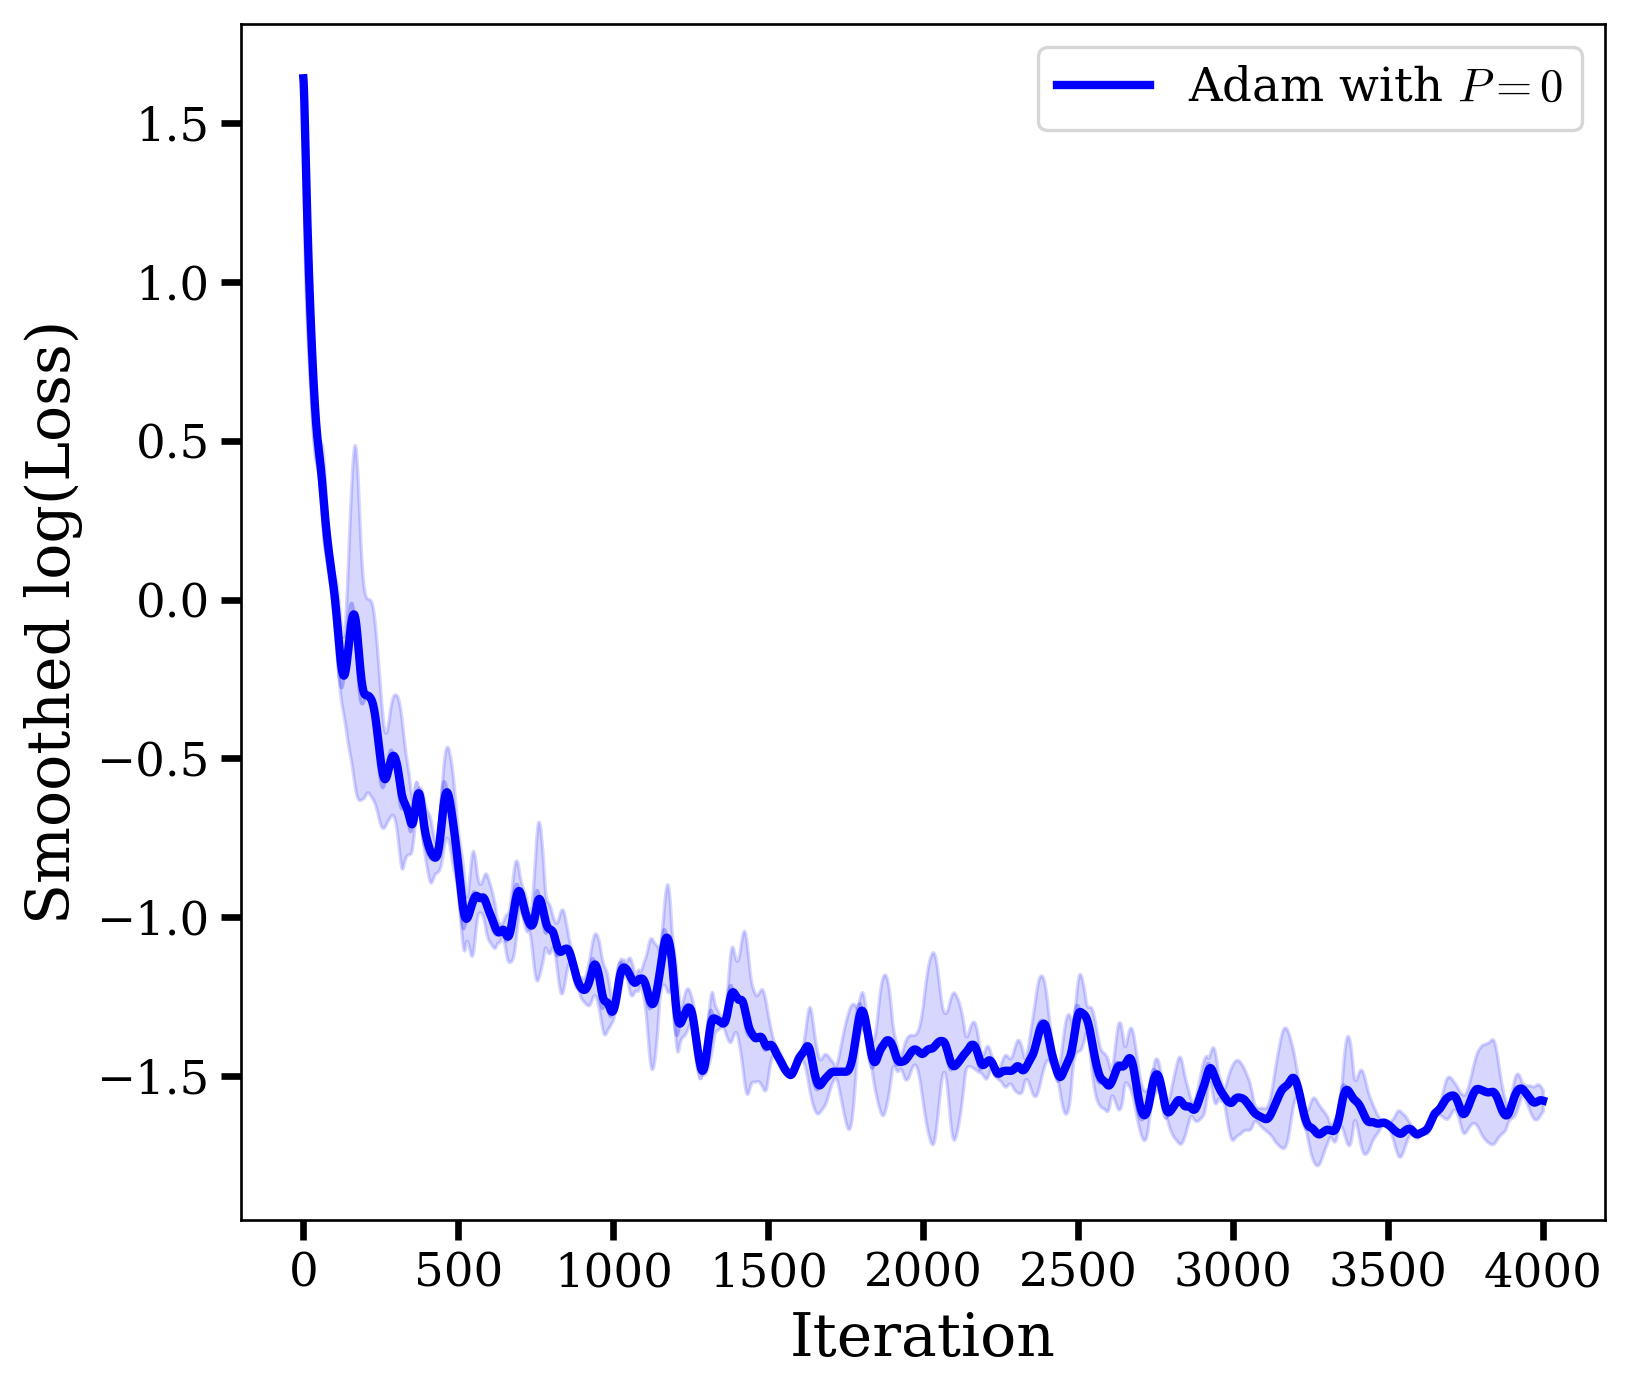
\includegraphics[width=\linewidth]{cre_t3_loss_smooth.png}
  \caption{CRE loss}
\end{subfigure}
\hfill
\begin{subfigure}{0.48\linewidth}
  \centering
  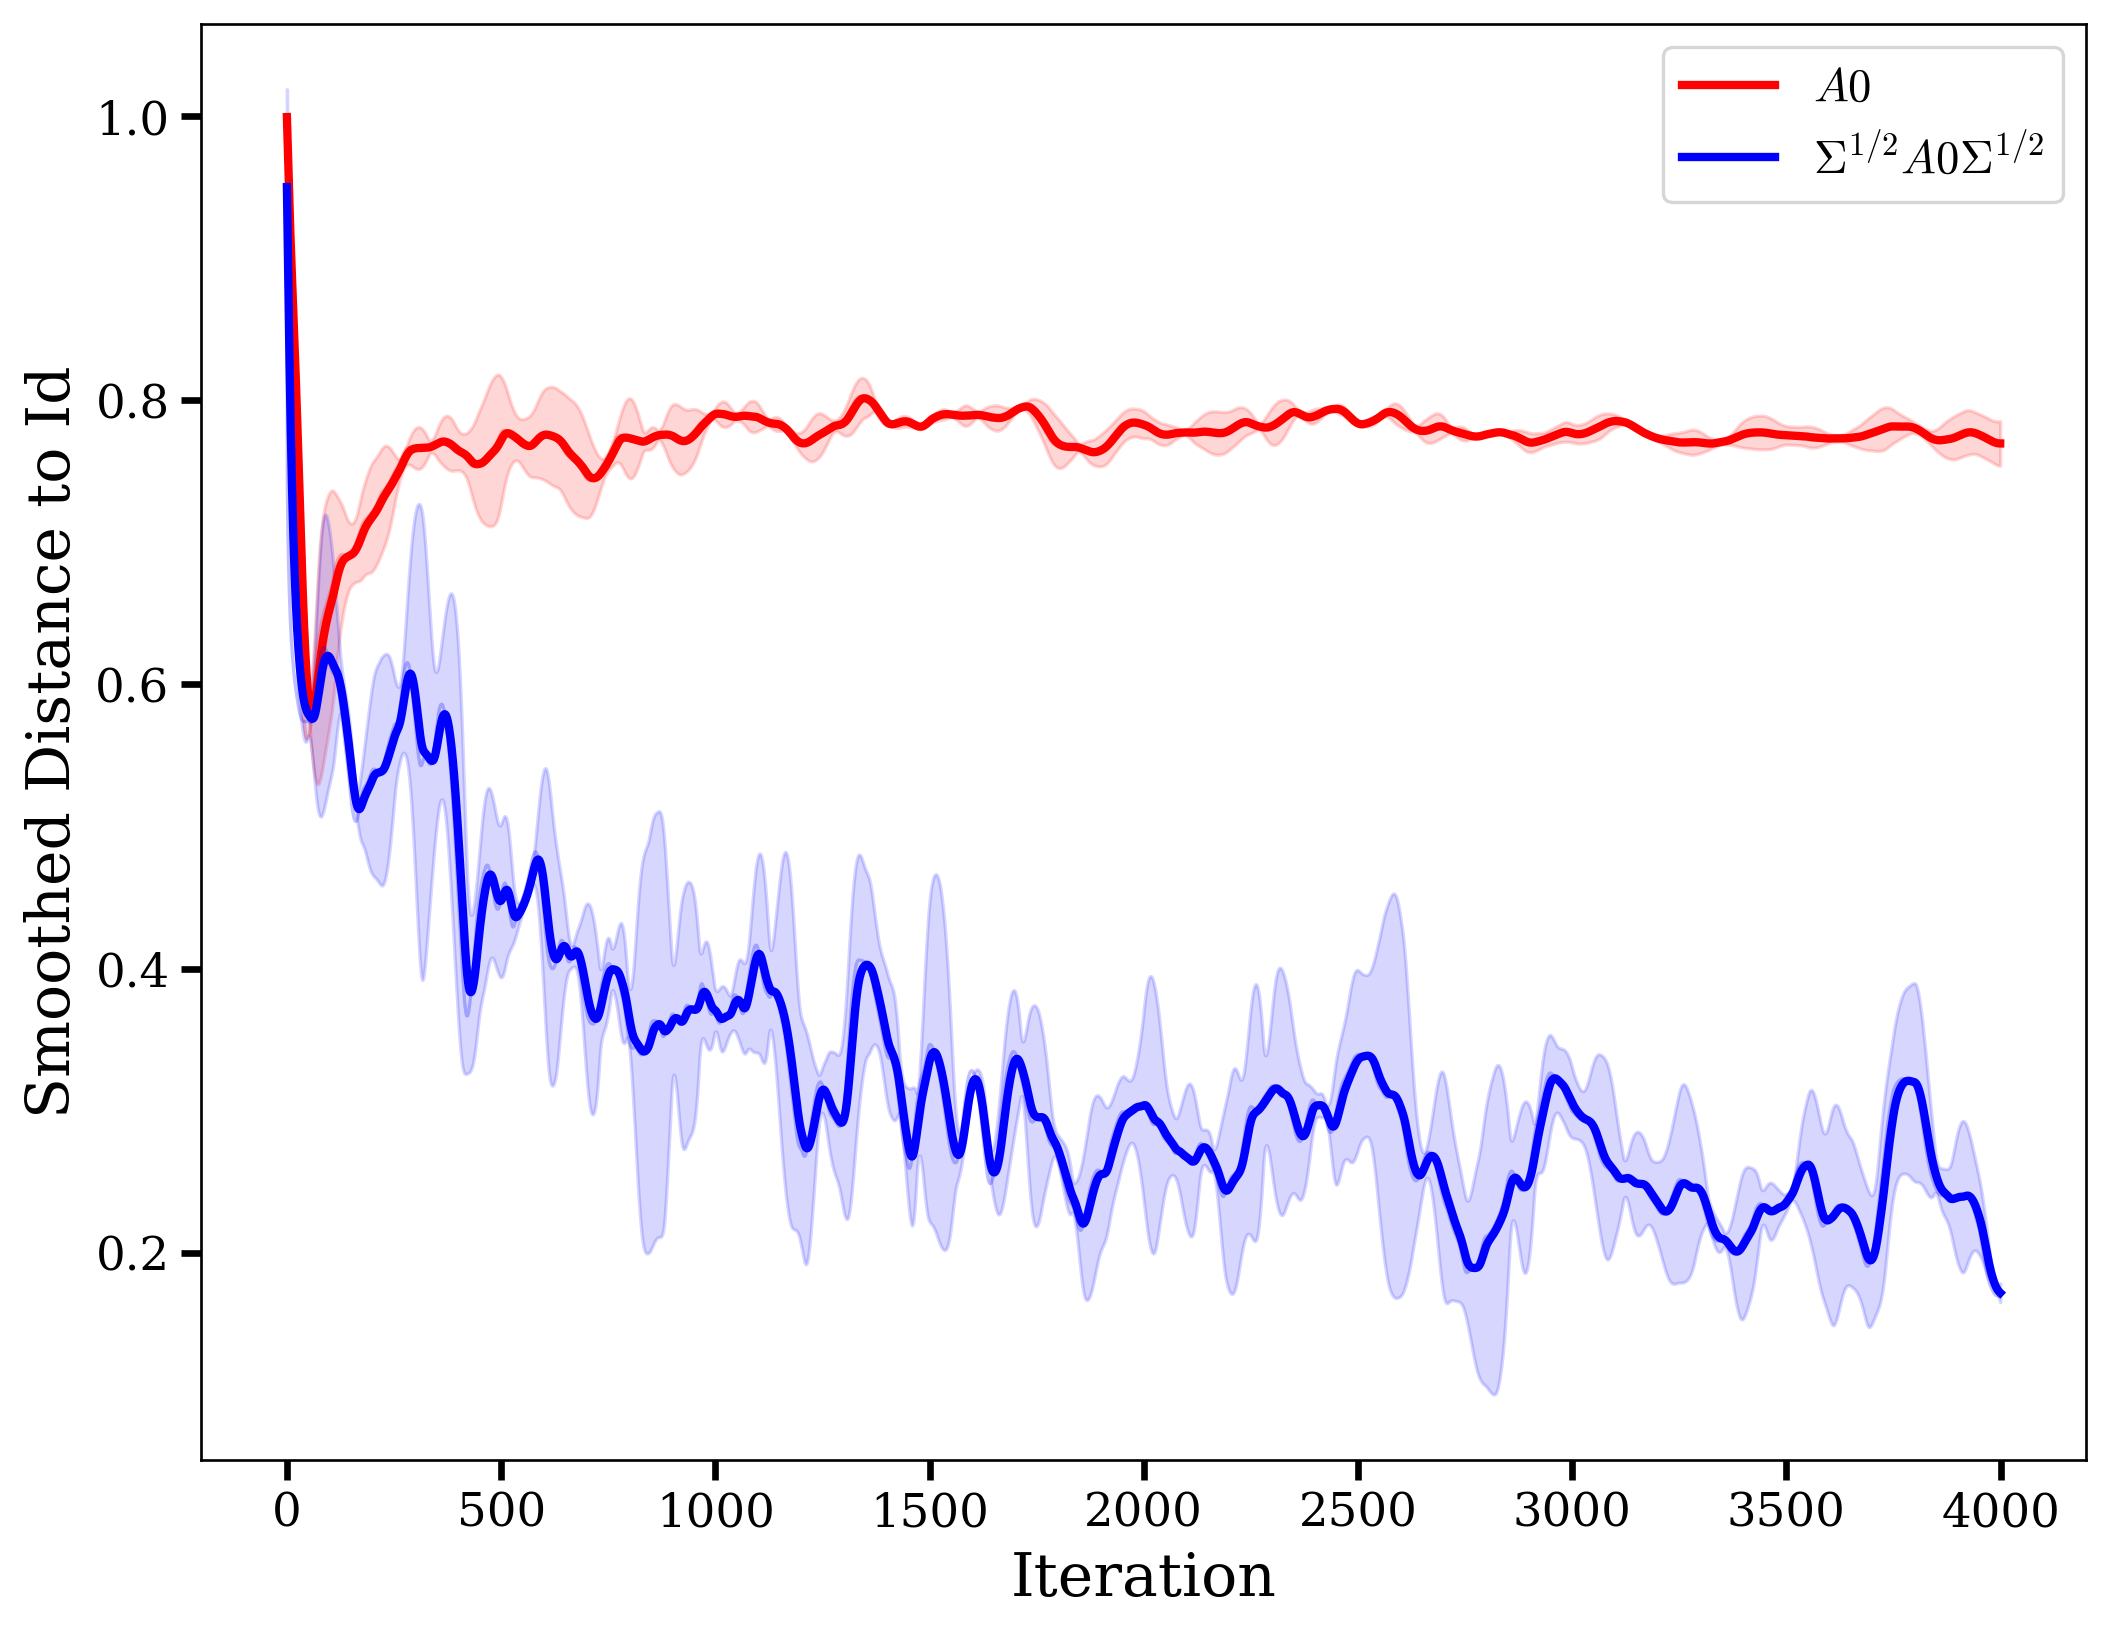
\includegraphics[width=\linewidth]{cre_t3_a0_distance_smooth.png}
  \caption{CRE $A_0$ 距离}
\end{subfigure}
\caption{Theorem 3 的 CRE 证据。课程规模实验保留了关键定性模式：loss 下降，旋转矩阵明显接近缩放单位阵。}
\label{fig:cre_t3}
\end{figure}

\begin{figure}[!t]
  \centering
  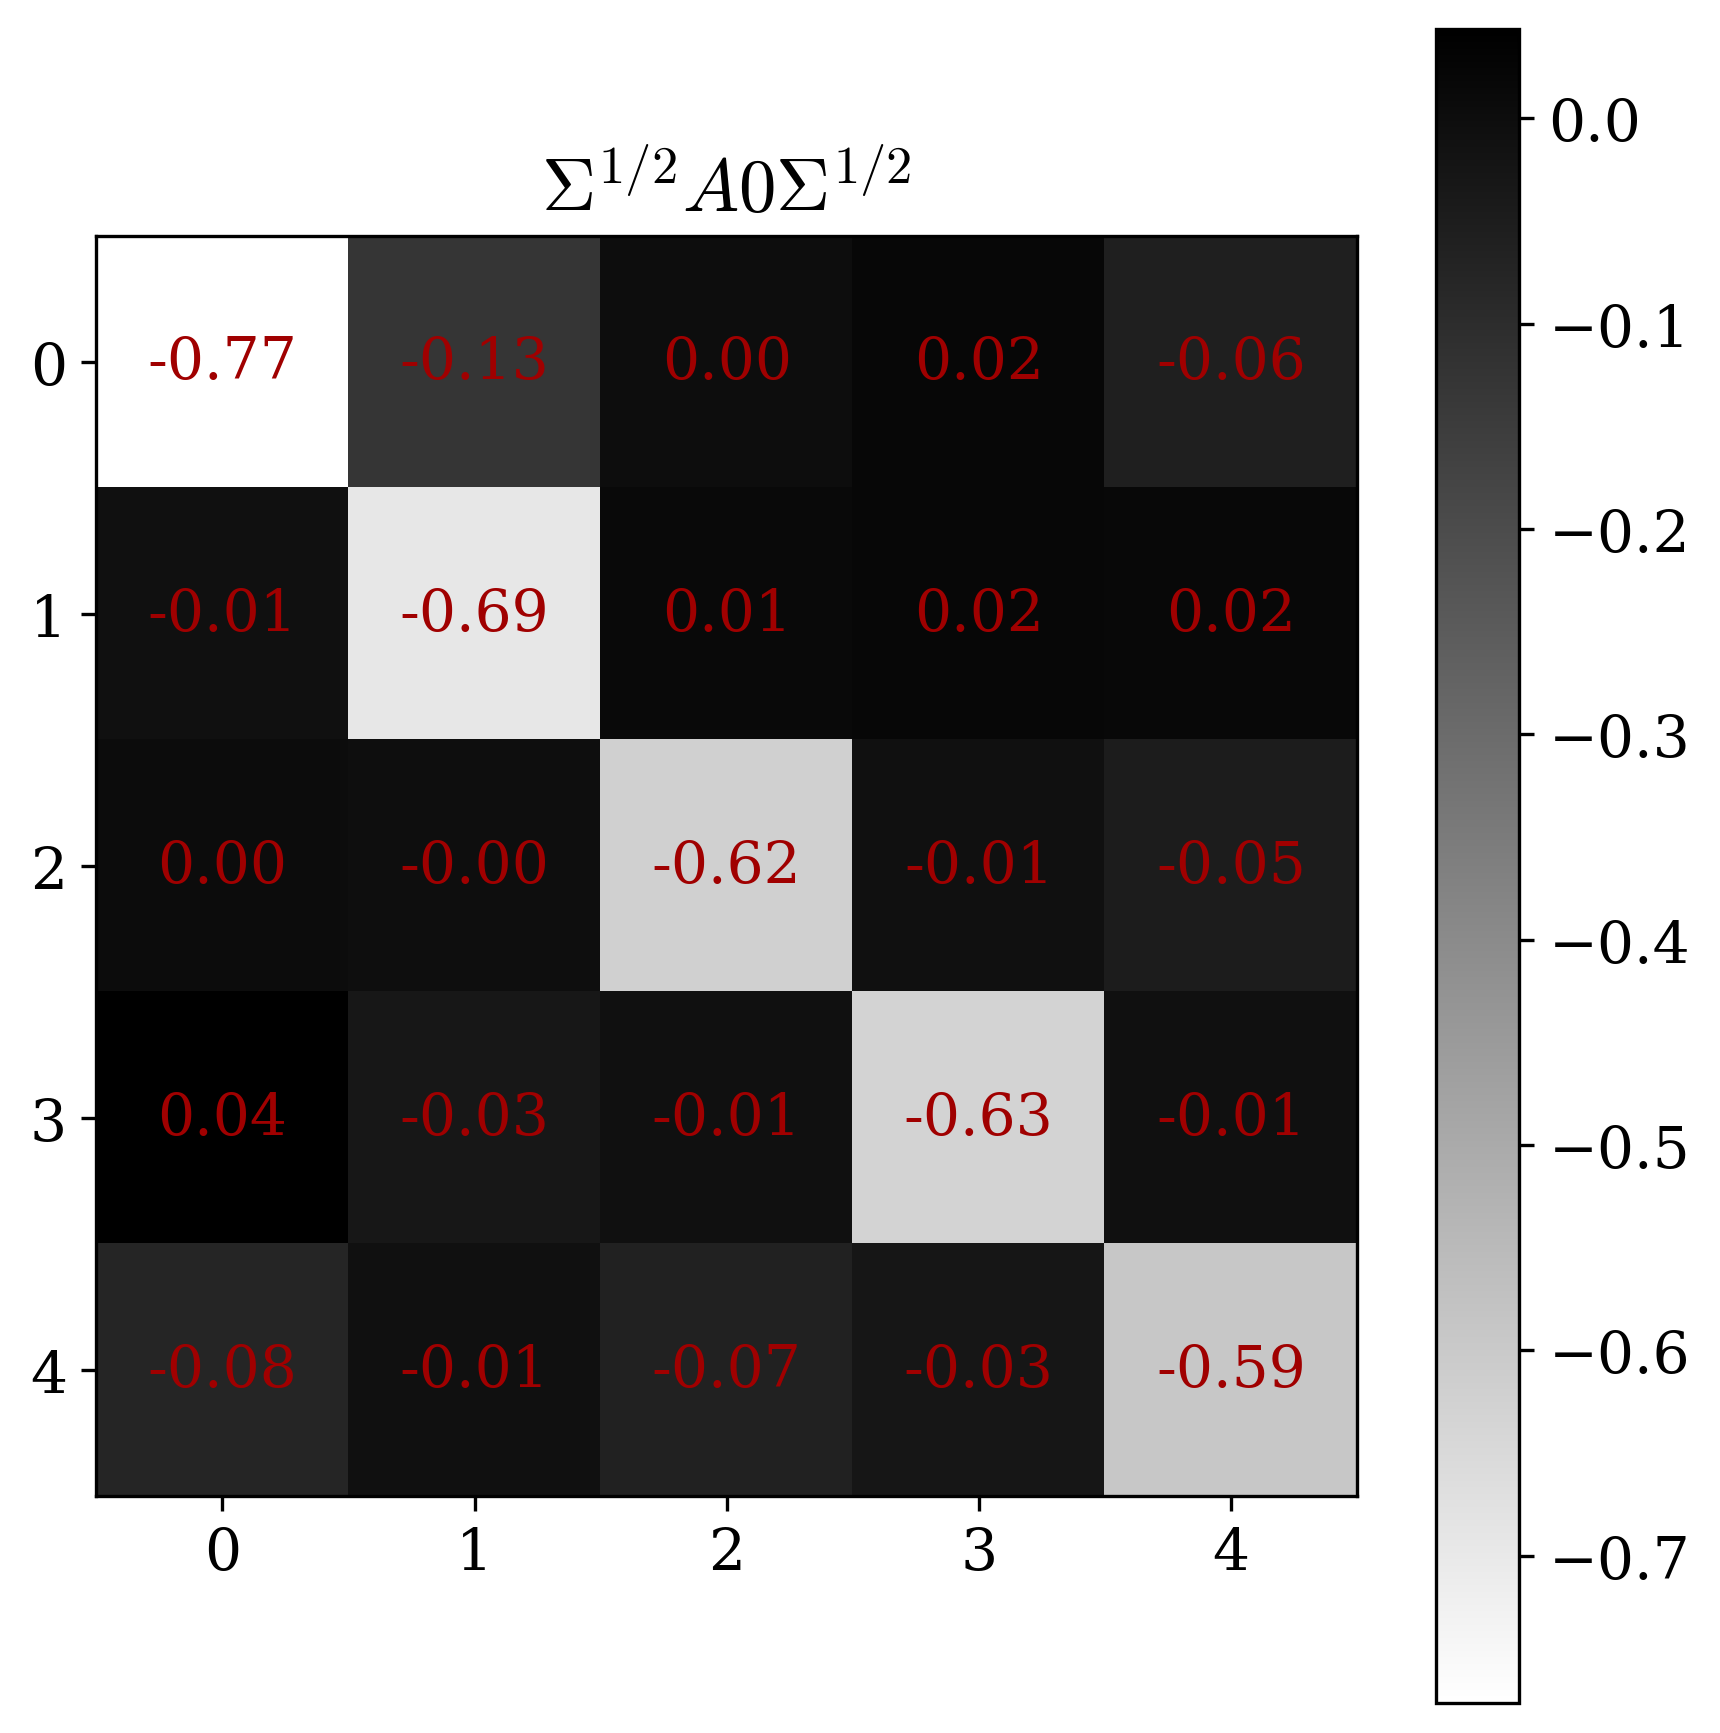
\includegraphics[width=0.72\linewidth]{cre_t3_a0_heatmap.png}
  \caption{稀疏约束设置下 CRE 最终旋转 $A_0$ 热力图。}
  \label{fig:cre_t3_heatmap}
\end{figure}

\begin{figure}[!t]
  \centering
  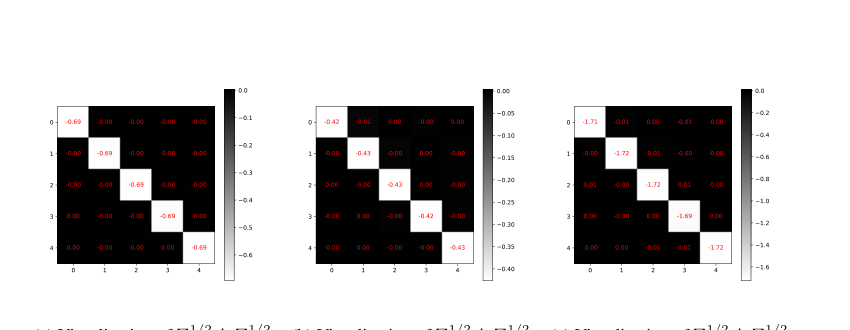
\includegraphics[width=\linewidth]{pse_theorem3_heatmaps.png}
  \caption{Theorem 3 的 PSE 最终热力图。这些图像是 CRE 热力图检查的参照。}
  \label{fig:pse_t3_heatmap}
\end{figure}

\subsection{Theorem 4：放宽约束下的特征变换}
Theorem 4 预测，在放宽参数后，模型可以同时学习预条件梯度步和特征变换。图 \ref{fig:pse_t4} 中的 PSE 证据显示 $B_i$ 与旋转 $A_i$ 的距离下降；图 \ref{fig:pse_t4_heatmap} 中的热力图显示 $B_0,B_1$ 接近缩放单位阵。

\begin{figure}[!t]
  \centering
  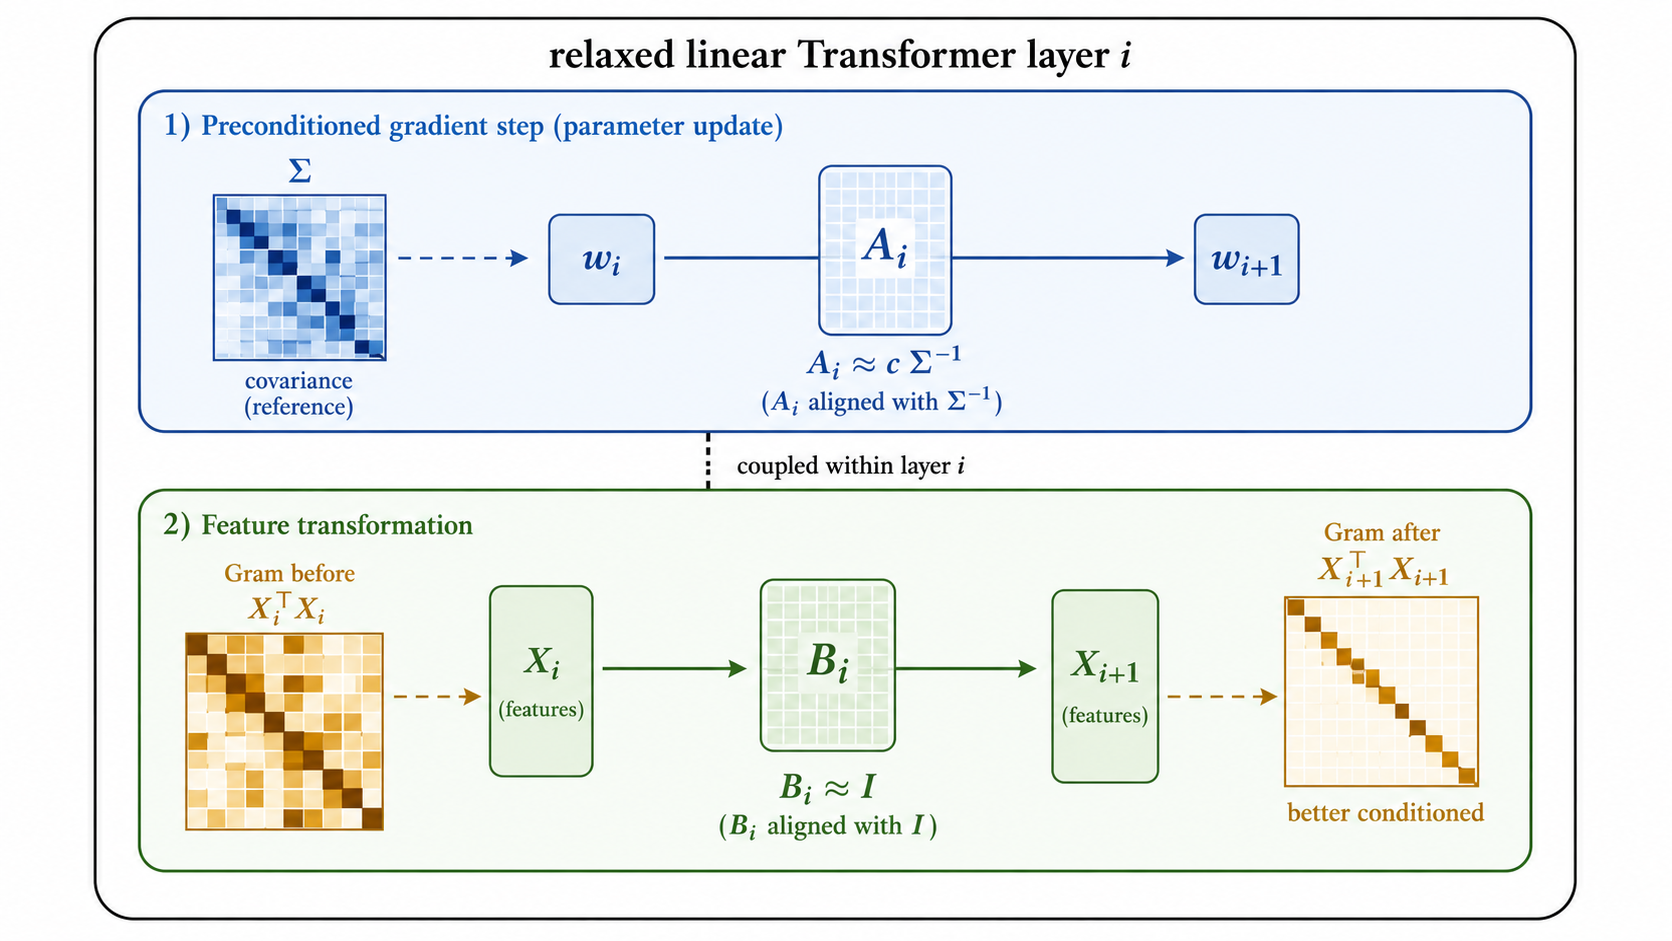
\includegraphics[width=\linewidth]{ai_theorem4_feature_transformation.png}
  \caption{Theorem 4 机制概念图。放宽模型通过 $A_i$ 执行预条件更新，并通过 $B_i$ 执行特征变换。}
  \label{fig:ai_t4}
\end{figure}

\begin{figure}[!t]
  \centering
  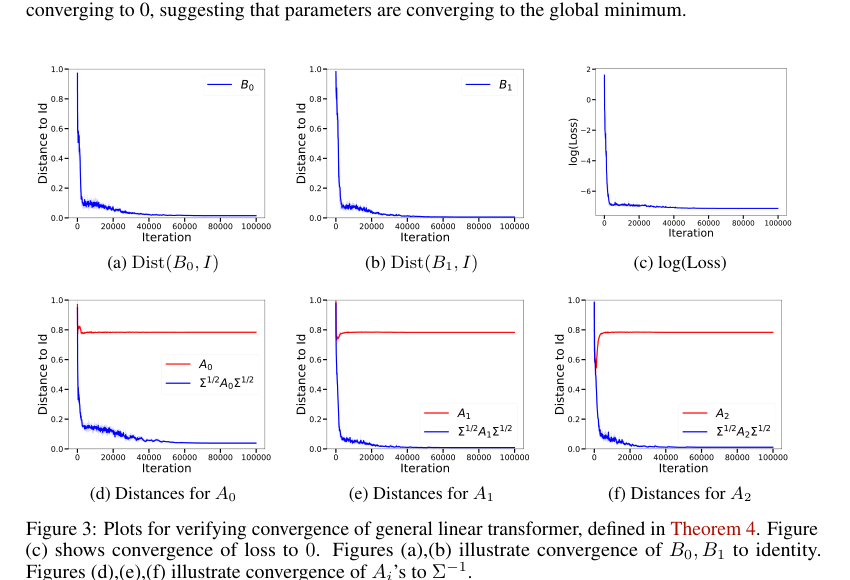
\includegraphics[width=\linewidth]{pse_theorem4_curves.png}
  \caption{Theorem 4 放宽参数设置下的 PSE 曲线。}
  \label{fig:pse_t4}
\end{figure}

\begin{figure}[!t]
  \centering
  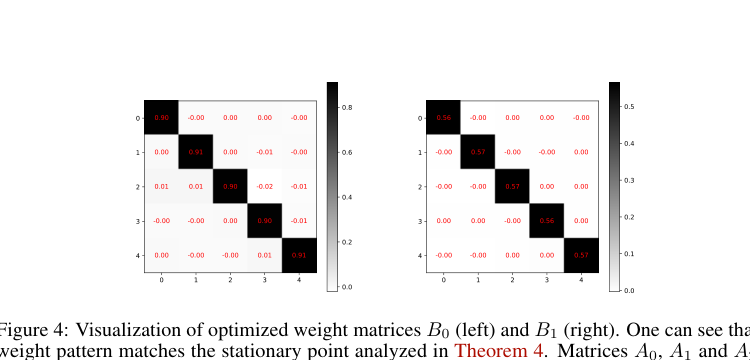
\includegraphics[width=\linewidth]{pse_theorem4_b_heatmaps.png}
  \caption{Theorem 4 中学习到的 $B_i$ 矩阵 PSE 热力图。}
  \label{fig:pse_t4_heatmap}
\end{figure}

CRE 运行也呈现了理论预期方向。log loss 从 $1.641430$ 降至 $-4.221714$。结构距离同样下降：$B_0$ 从 $0.997822$ 降至 $0.558772$，$B_1$ 从 $0.966573$ 降至 $0.477783$，$A_0$ 从 $0.950218$ 降至 $0.373056$，$A_1$ 从 $0.975746$ 降至 $0.376785$，$A_2$ 从 $0.965415$ 降至 $0.394170$。这些曲线不用于声明完全达到论文规模数值，但复现了关键结构趋势。

放宽设置比稀疏设置理论上更丰富，因为模型不再被迫固定特征行。从优化角度看，这意味着网络同时学习更新规则和表示变换。表示变换可以改善后续层看到的 Gram 矩阵条件数。因此，训练出的过程更像带内部状态变换的学习优化器，而不是固定手写梯度方法。

\begin{table}[!t]
\centering
\caption{CRE Theorem 4 结构指标。}
\label{tab:t4_metrics}
\begin{tabular}{lrrr}
\toprule
指标 & 初始 & 最终 & 变化\\
\midrule
Log loss & 1.6414 & -4.2217 & -5.8631\\
$B_0$ 距离 & 0.9978 & 0.5588 & -0.4391\\
$B_1$ 距离 & 0.9666 & 0.4778 & -0.4888\\
$A_0$ 距离 & 0.9502 & 0.3731 & -0.5772\\
$A_1$ 距离 & 0.9757 & 0.3768 & -0.5990\\
$A_2$ 距离 & 0.9654 & 0.3942 & -0.5712\\
\bottomrule
\end{tabular}
\end{table}

\begin{figure}[!t]
\centering
\begin{subfigure}{0.48\linewidth}
  \centering
  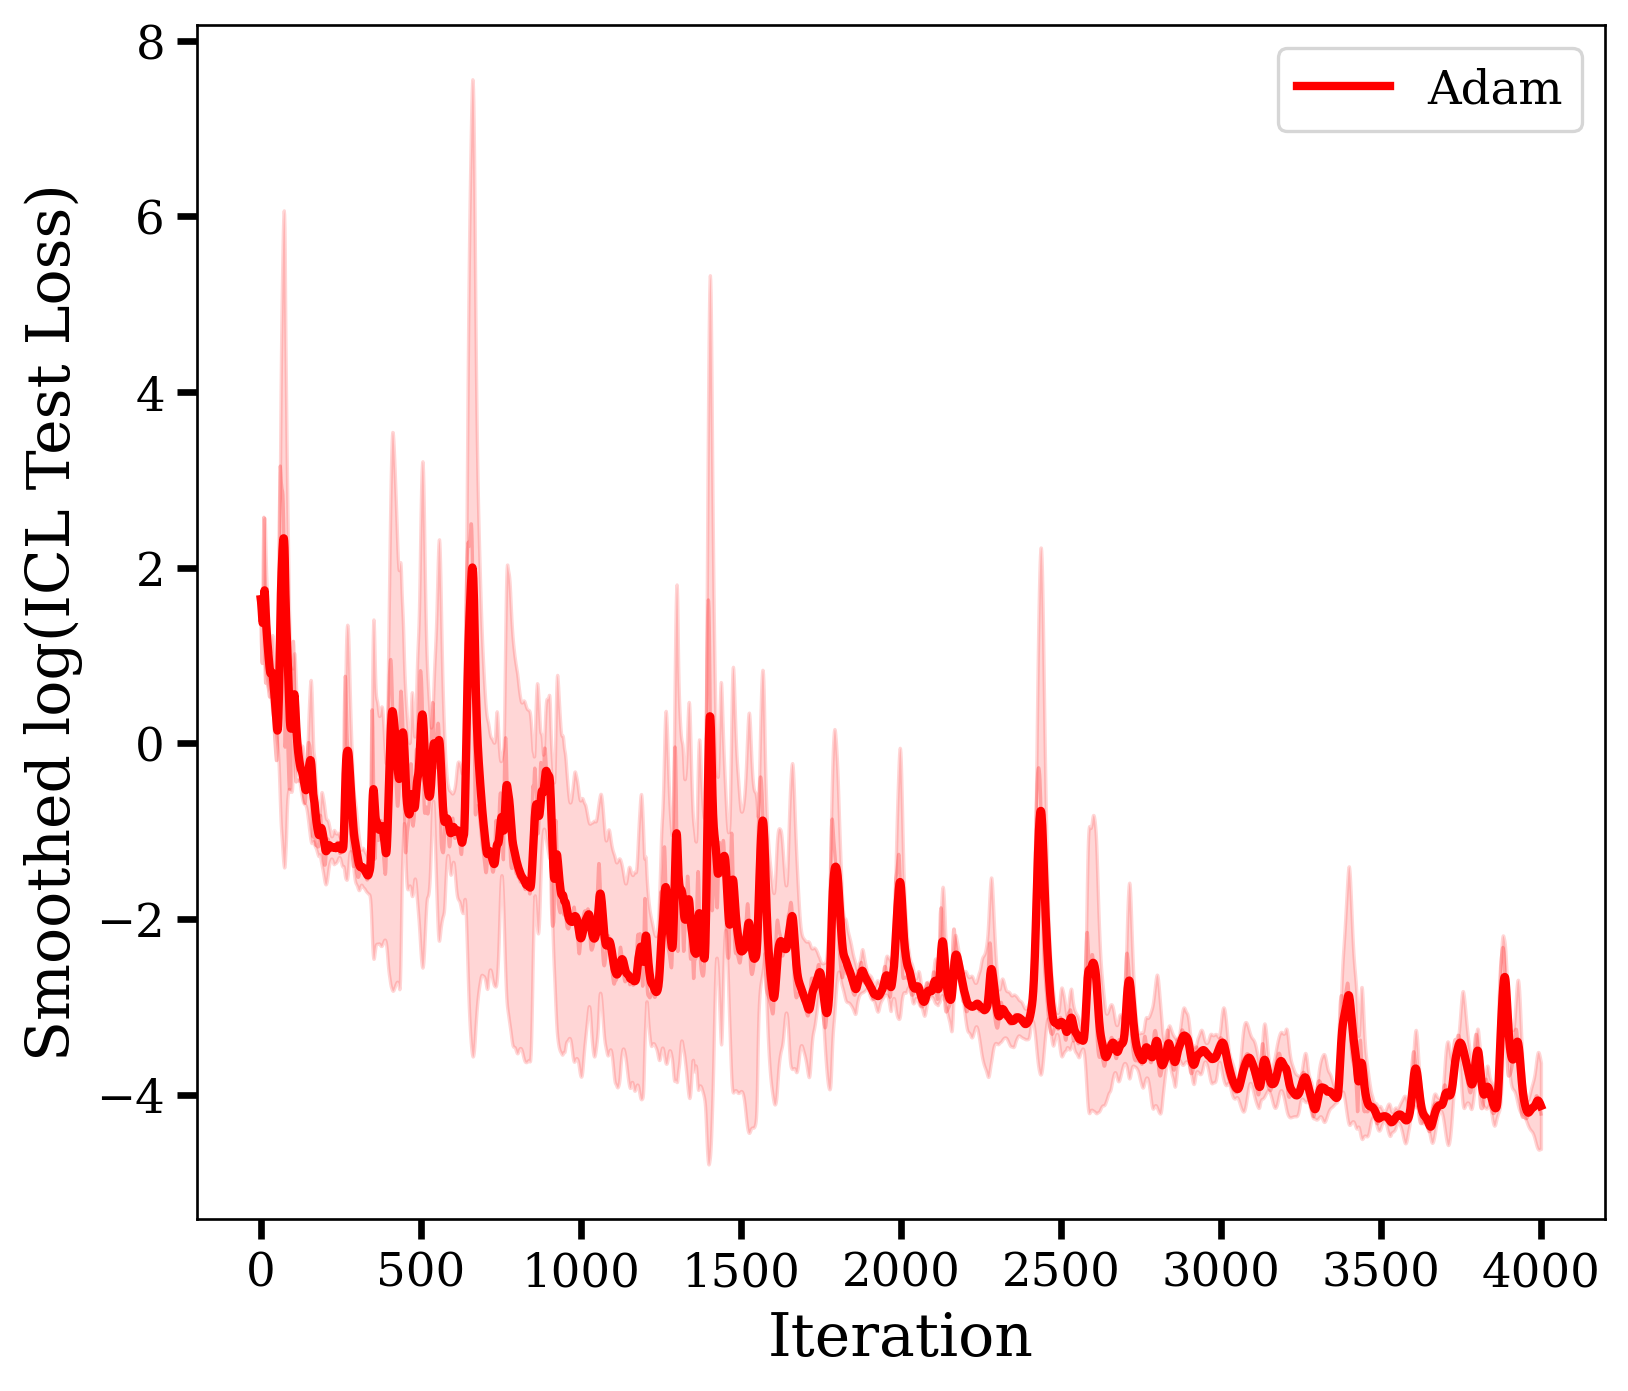
\includegraphics[width=\linewidth]{cre_t4_loss_smooth.png}
  \caption{CRE loss}
\end{subfigure}
\hfill
\begin{subfigure}{0.48\linewidth}
  \centering
  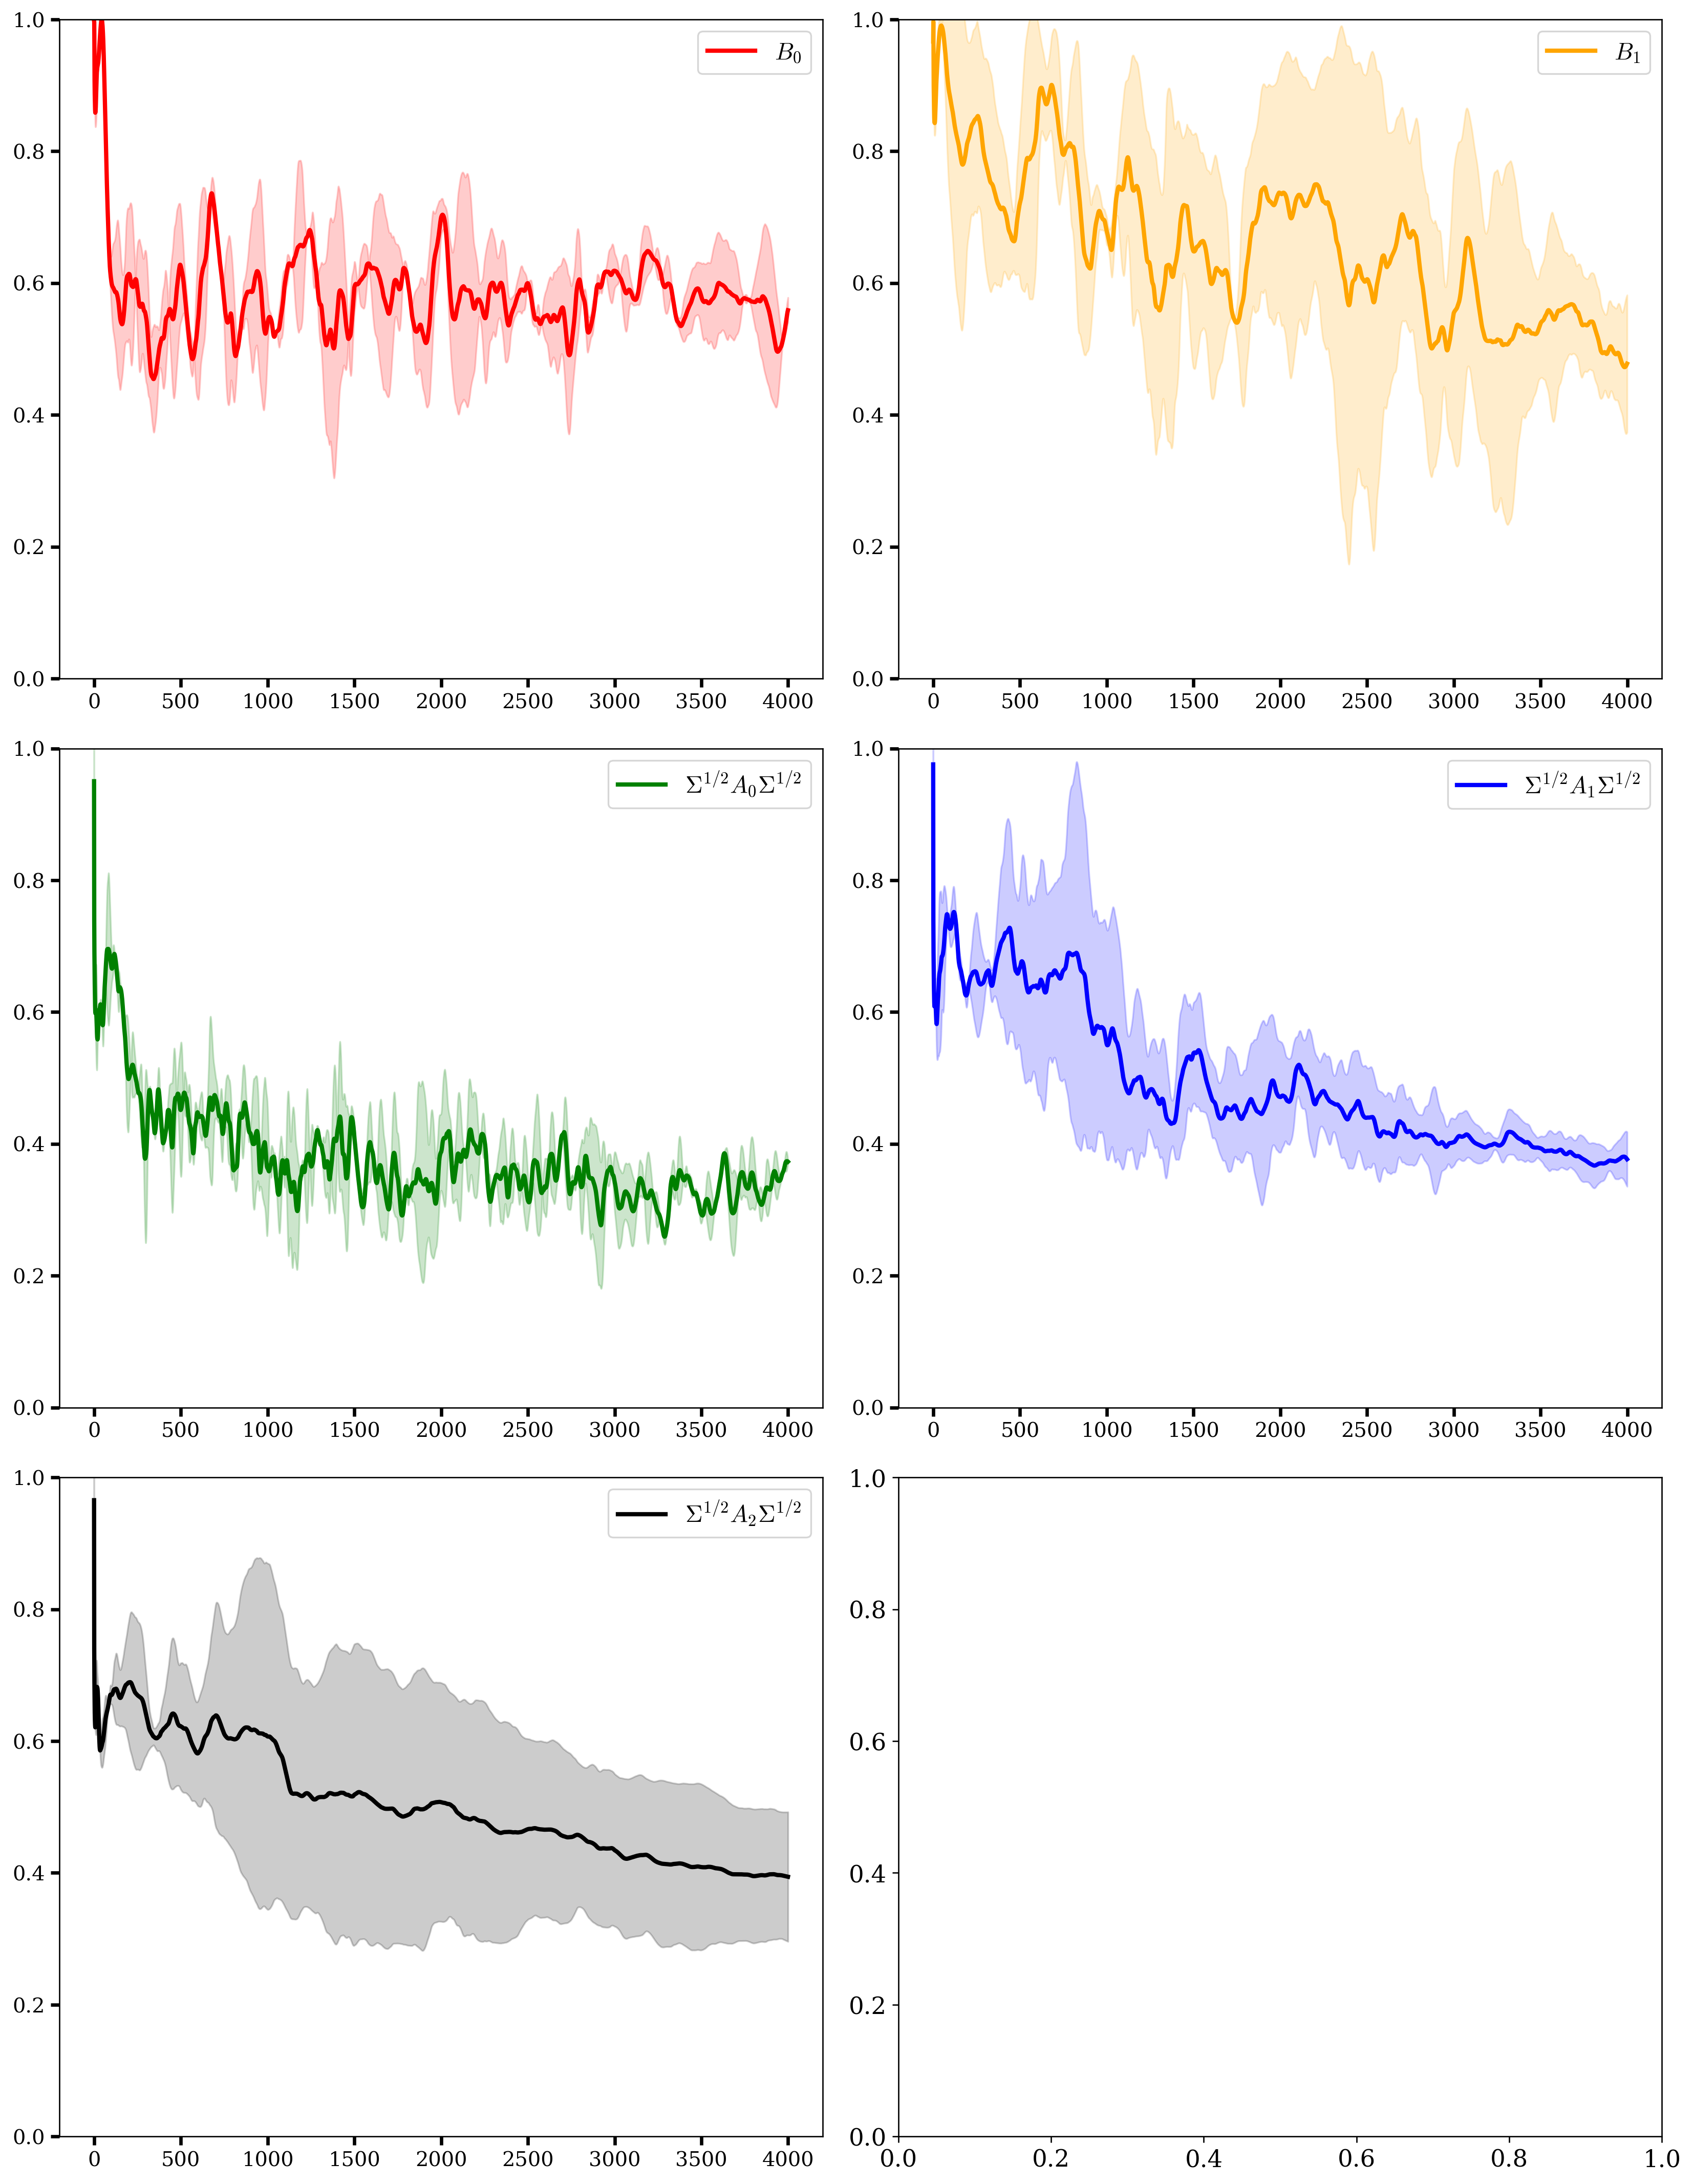
\includegraphics[width=\linewidth]{cre_t4_distance_panel.png}
  \caption{CRE 距离面板}
\end{subfigure}
\caption{Theorem 4 的 CRE 证据。loss 与结构距离均朝放宽临界点理论预测方向变化。}
\label{fig:cre_t4}
\end{figure}

\begin{figure}[!t]
  \centering
  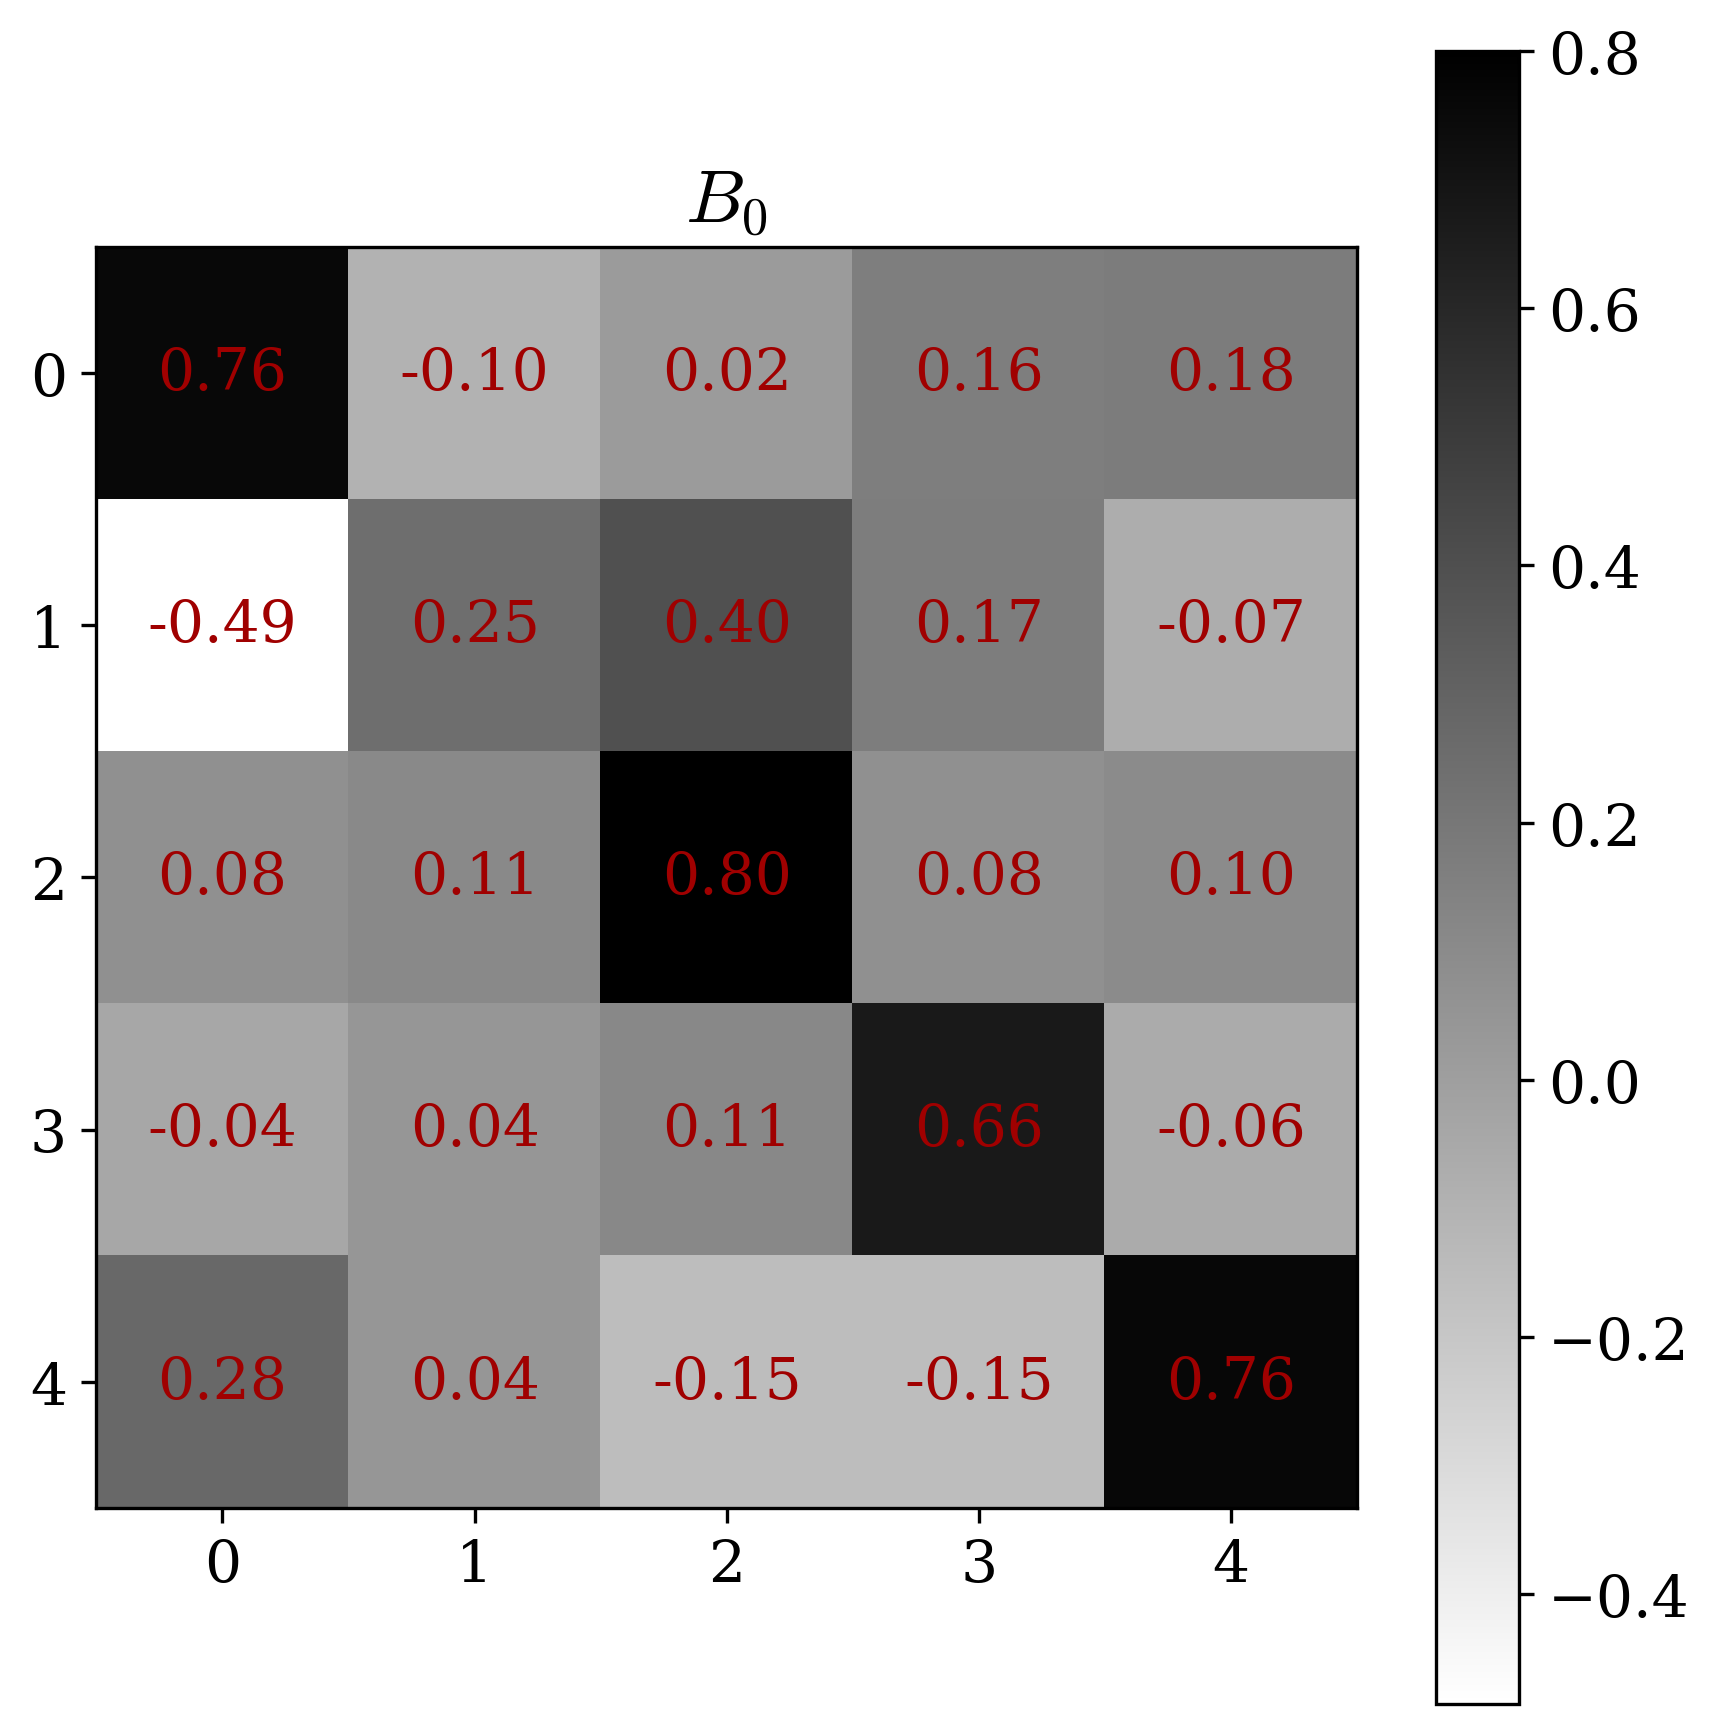
\includegraphics[width=0.72\linewidth]{cre_t4_b0_heatmap.png}
  \caption{放宽设置下 CRE 最终 $B_0$ 热力图。}
  \label{fig:cre_t4_heatmap}
\end{figure}

\section{扩展实验：上下文长度}
上下文长度实验提供了样本复杂度视角。Prompt 中样本越多，各方法能够获得的任务信息越充分。图 \ref{fig:variable_n} 比较了三层线性 Transformer、三步 GD、三步预条件 GD 和 OLS 在不同上下文长度下的测试损失。

\begin{figure}[!t]
  \centering
  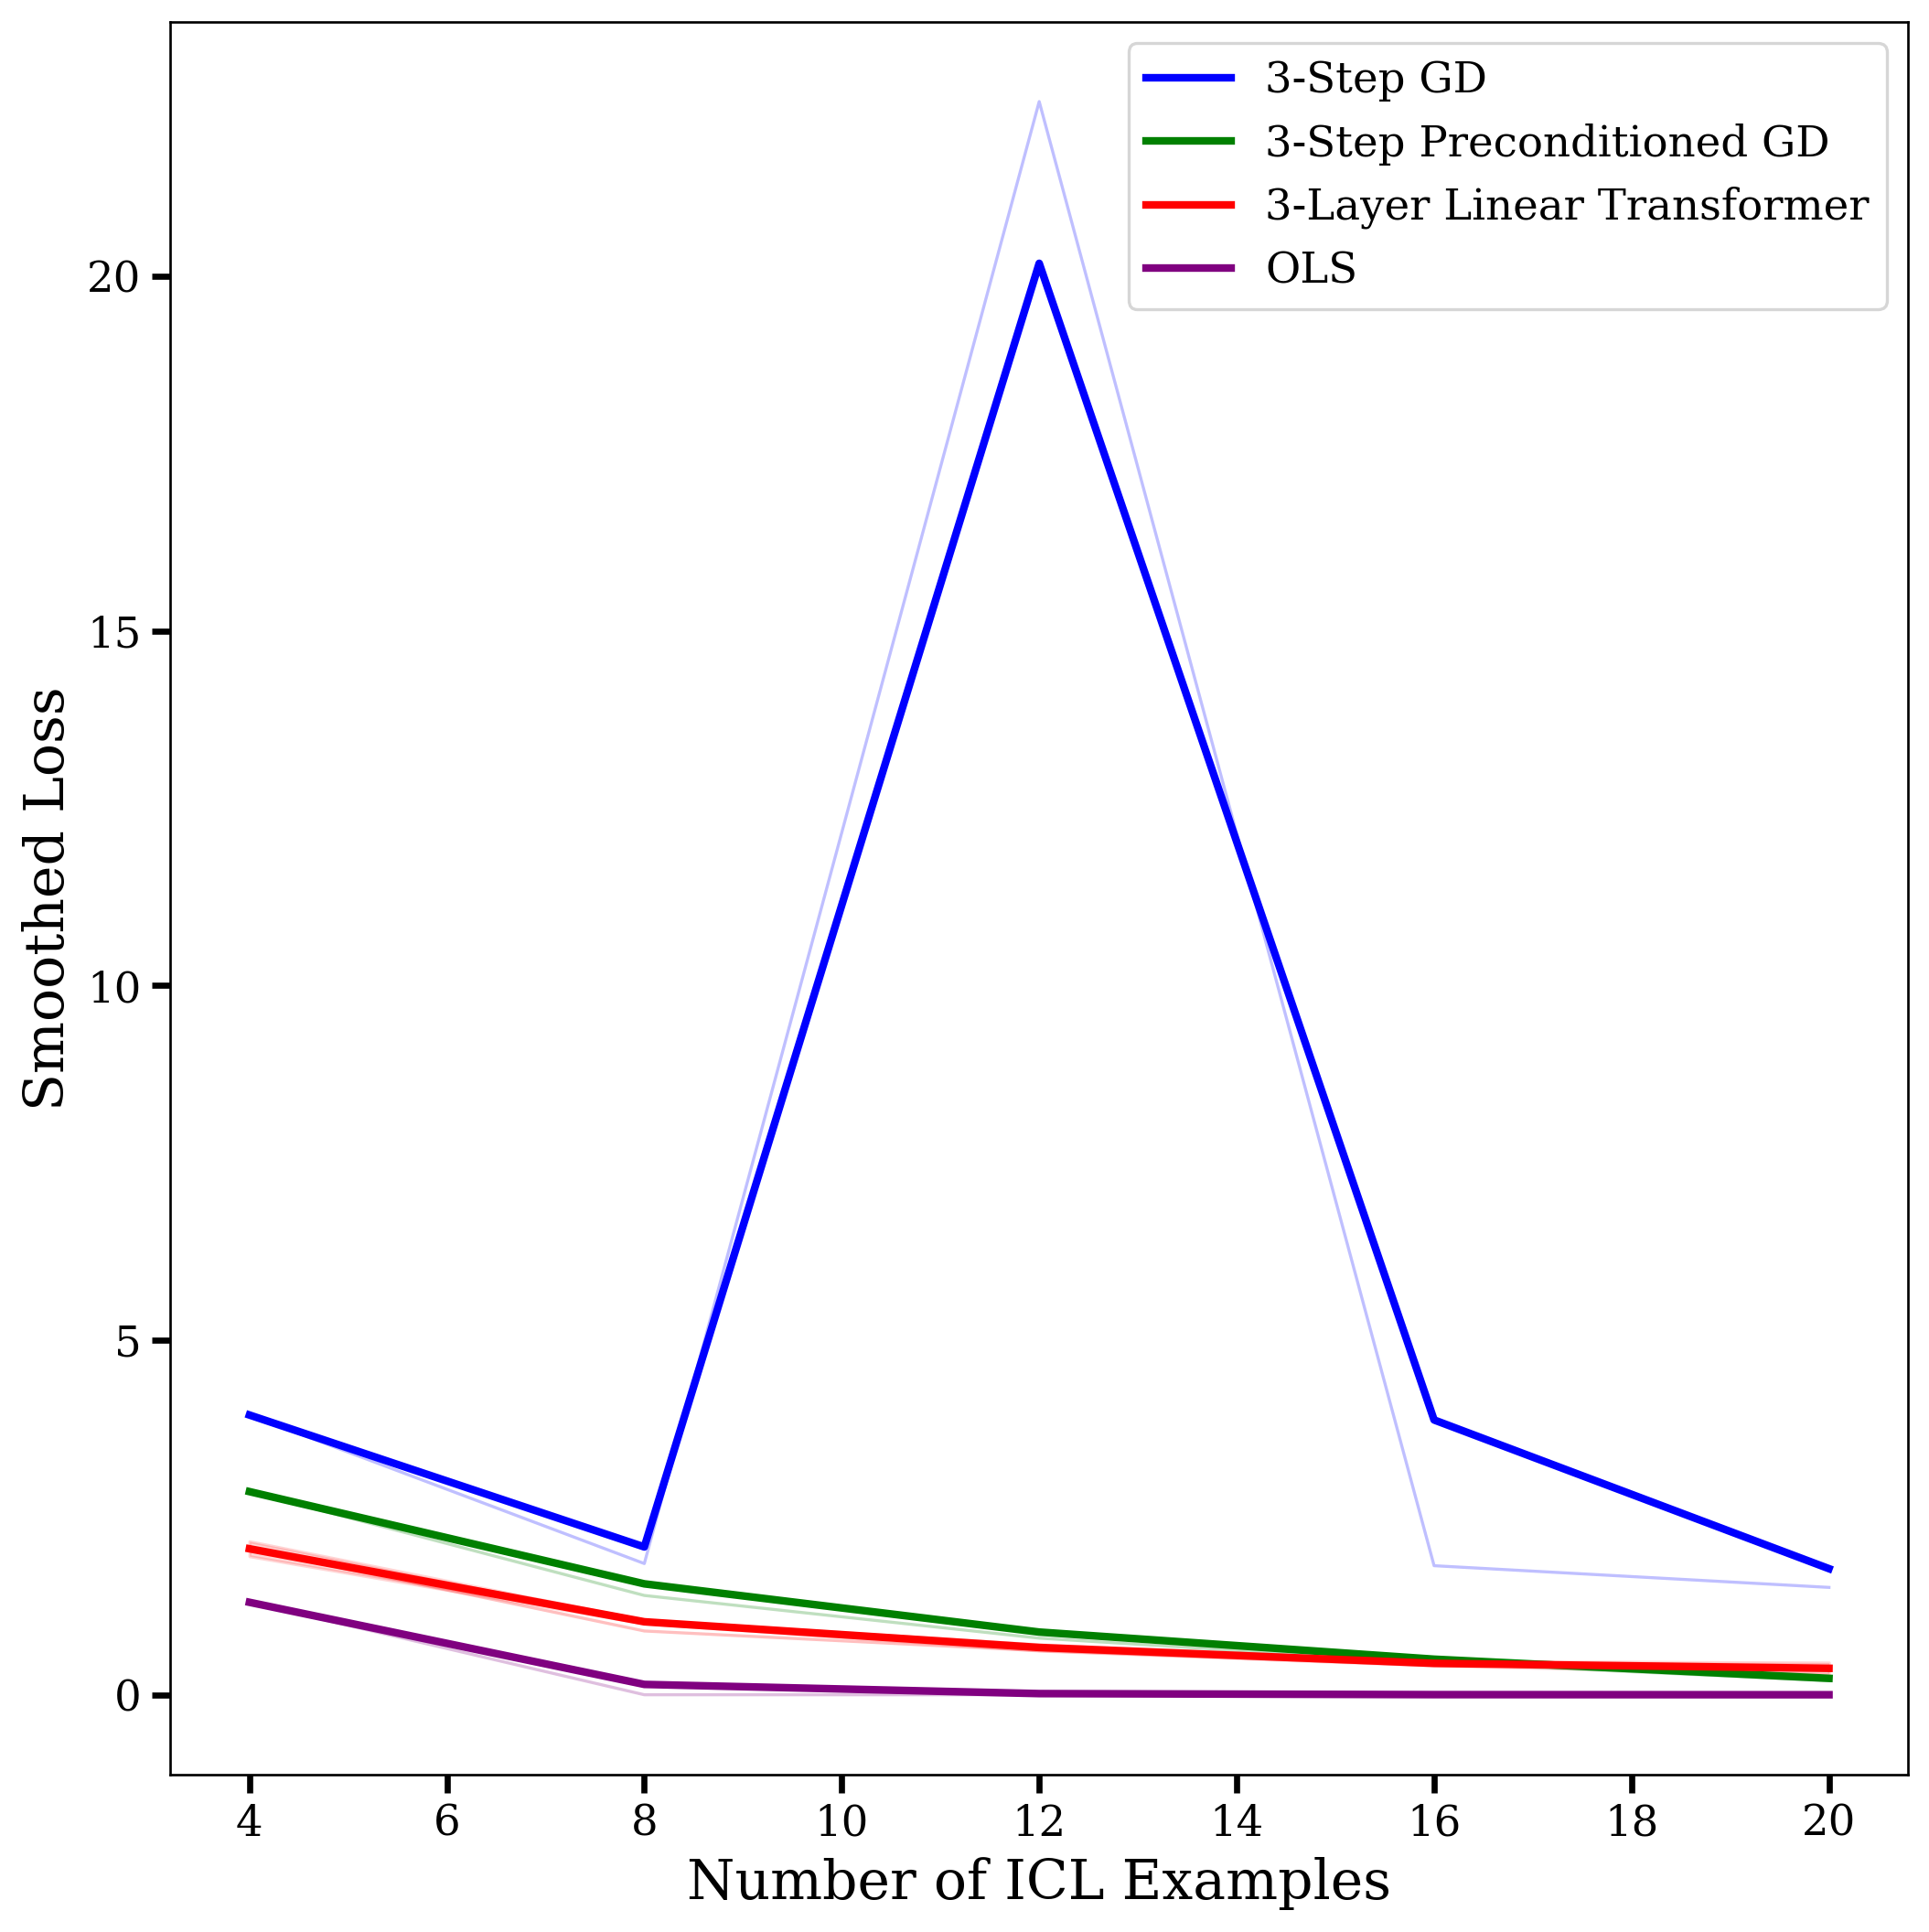
\includegraphics[width=\linewidth]{cre_variable_n_smooth.png}
  \caption{CRE 上下文长度扩展实验。随着上下文样本数增加，测试损失整体改善。}
  \label{fig:variable_n}
\end{figure}

\begin{table}[!t]
\centering
\caption{CRE 上下文长度实验摘要。数值为平均测试损失。}
\label{tab:variable_n}
\begin{tabular}{rrrrr}
\toprule
$N$ & Transformer & GD & PGD & OLS\\
\midrule
4 & 2.0586 & 3.9445 & 2.8644 & 1.3038\\
8 & 0.8993 & 1.8499 & 1.4001 & 0.0000\\
12 & 0.6211 & 22.4652 & 0.7983 & 0.0000\\
16 & 0.4147 & 1.8198 & 0.4534 & 0.0000\\
20 & 0.3640 & 1.5138 & 0.1976 & 0.0000\\
\bottomrule
\end{tabular}
\end{table}

Transformer loss 从 $N=4$ 时的 $2.058553$ 降至 $N=20$ 时的 $0.363965$。预条件 GD 也从 $2.864391$ 降至 $0.197570$。当上下文样本充足时，OLS 接近精确解。图中 $N=12$ 处可见的特殊突刺主要来自普通 GD 曲线，而不是 Transformer 主趋势。该突刺更适合解释为有限步优化的数值敏感性：在只有三步 GD、步长通过有限网格选择、且输入协方差非各向同性的情况下，未预条件的固定步长更新可能在某个上下文长度上放大病态方向或发生过冲。相比之下，PGD 没有出现同等级突刺，这反而支持论文主线：协方差感知的预条件可以稳定优化。该扩展实验强化了主线结论：预条件对优化过程很重要，而更多上下文样本可以降低任务不确定性。

该比较也澄清了 Transformer 的角色。训练后的线性 Transformer 不一定总是最优估计器；当样本足够时，OLS 是很强的闭式解参考。Transformer 结果的价值在于机制解释：它说明训练后的 attention 模型可以从 prompt 数据中近似一个迭代优化器。因此 variable-$N$ 实验是对 Theorem 3 和 Theorem 4 结构实验的补充，而不是替代。

\subsection{偏差-方差与算法效率}
上下文长度实验也可以从偏差-方差角度理解。当样本很少时，各方法都难以准确恢复 $\wstar$。OLS 偏差低，但在信息不足或方程欠定时可能不稳定。梯度类方法则通过步数和步长选择引入算法偏差。预条件 GD 改变了这种偏差，因为它根据协方差调整更新几何。训练后的 Transformer 也具有类似算法限制：层数固定时，它只能执行固定次数的学习到的更新。

因此，有限深度 Transformer 可以看成一种计算受限估计器。增加 $N$ 提高了统计信息量，但在 CRE 实验中模型仍然只有三步学习到的更新。loss 随 $N$ 下降说明该迭代计算能利用更多上下文样本；与 OLS 的差距则说明有限深度学习优化并不等同于精确求解完整最小二乘问题。

\section{讨论}
论文的核心贡献是把 ICL 解释从表达能力推进到训练诱导的算法结构。人工构造权重可以模拟梯度下降是一类表达性结论；证明训练目标的全局最优点或近似临界点具有梯度法形式，则更接近学习理论中的优化景观分析。

本项目复现支持结构层面的理论结论。Theorem 3 的关键不只是 loss 下降，而是协方差调整后的矩阵比原始矩阵更接近缩放单位阵。Theorem 4 中，$A_i$ 和 $B_i$ 的共同变化支持“放宽线性 attention 能学习超出标准梯度下降的特征变换机制”这一解释。上下文长度扩展实验则补充比较了 Transformer、GD、预条件 GD 与 OLS 在样本数变化下的行为。

局限性也需要明确。论文分析适用于线性 attention、高斯线性回归任务和特定参数结构，不能直接推广为所有大语言模型都以相同方式执行梯度下降。论文也没有完全刻画非凸训练目标的所有临界点。CRE 的定位是验证趋势与结构一致性，而不是复现所有论文规模数值。

\subsection{潜在拓展}
后续可以从几个方向扩展。第一，最直接的理论扩展是分析 softmax attention。目标论文为了可解析性去掉了 softmax，但实际 Transformer 使用非线性 attention。第二，可以研究更丰富的任务分布，例如稀疏线性模型、非线性回归或分类任务。第三，复现实验可以增加随机种子和训练预算，以估计结构指标的方差。第四，可以继续分析论文中特定临界结构之外的 loss landscape，因为非凸目标可能包含多类不同性质的驻点。

\subsection{对学习理论的启示}
本项目展示了一种分析现代架构的学习理论路径：不把神经网络只看成黑盒预测器，而是追问训练诱导出了什么算法。如果训练后的模型实现了某种已知优化方法，那么条件数、步长、预条件器和样本数等经典概念就可以用来解释神经网络行为。这并没有解决 ICL 的完整理论，但为 Transformer 计算与优化理论之间建立了具体桥梁。

\begin{figure}[!t]
  \centering
  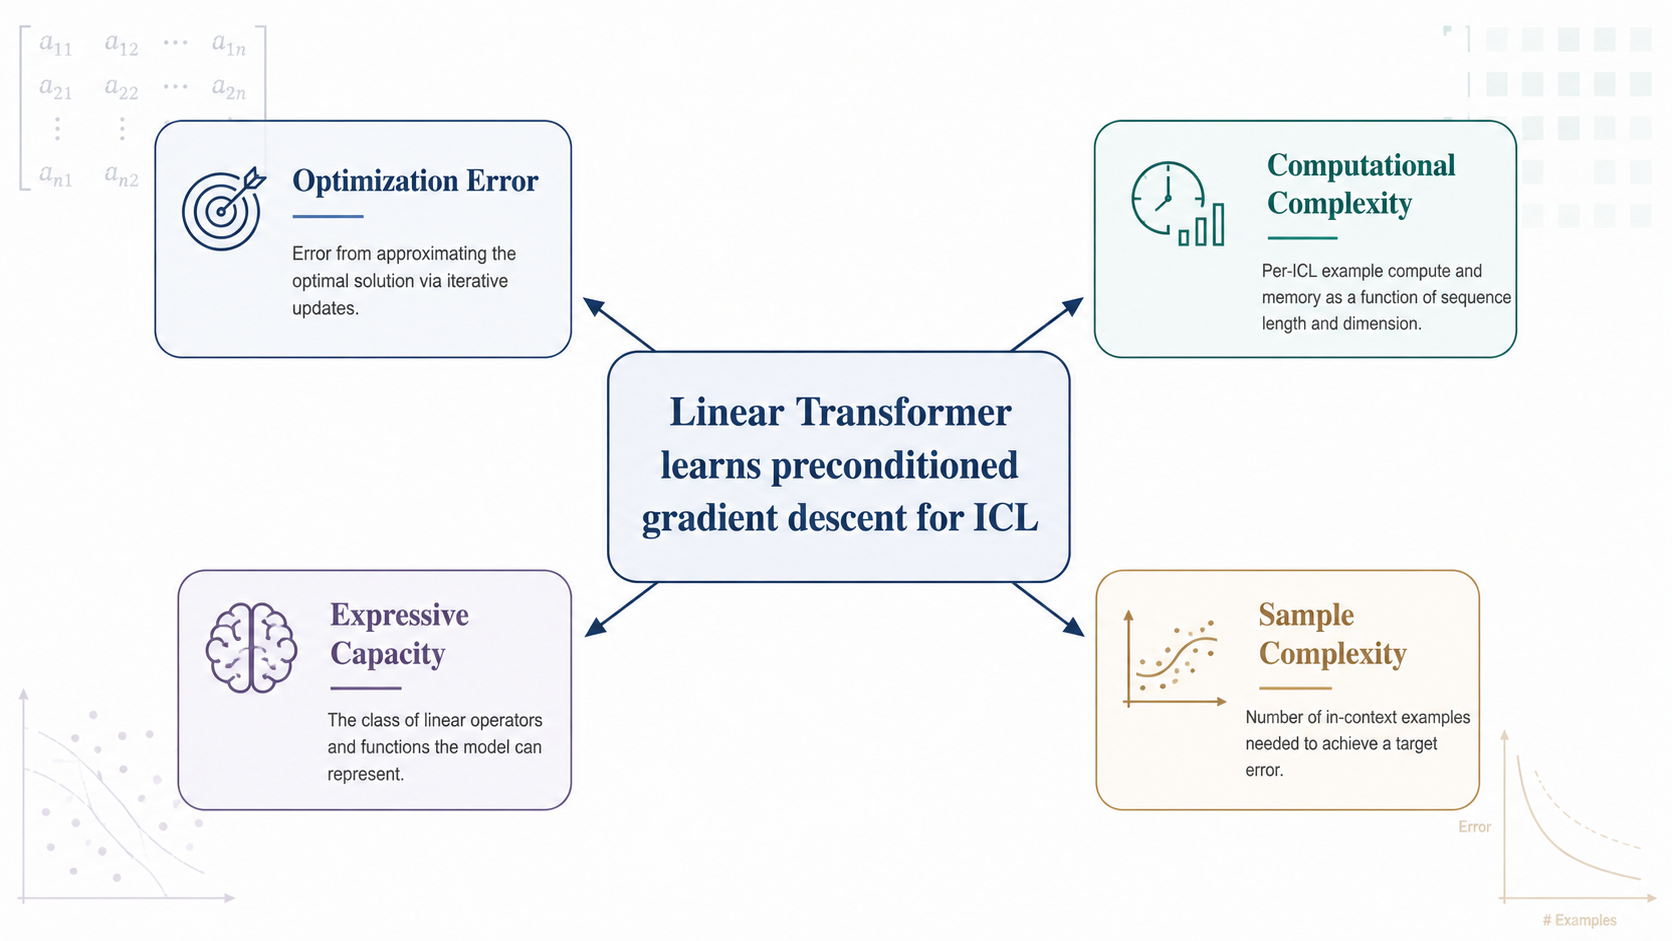
\includegraphics[width=\linewidth]{ai_summary.png}
  \caption{课程解释框架总结：优化误差、计算复杂度、表达能力与样本复杂度在 ICL 的学习优化视角中汇合。}
  \label{fig:ai_summary}
\end{figure}

\section{结论}
Ahn 等人的 NeurIPS 2023 论文给出了一个明确机制：训练后的线性 Transformer 可以在上下文学习中实现预条件梯度下降。其核心启示是，attention 层可以被解释为学习到的优化步骤；在放宽参数设置下，模型还可学习改善条件数的特征变换。本项目的课程规模复现确认了主要定性信号：上下文学习 loss 下降、旋转矩阵接近缩放单位阵、特征变换矩阵朝理论结构靠近，以及上下文样本数增加时测试损失改善。因此，该项目将优化误差、计算复杂度、表达能力和样本复杂度视角统一到一个有理论支撑的 Transformer 复现任务中。

\bibliographystyle{IEEEtran}
\bibliography{references}

\end{document}
